\documentclass[a4paper,12pt]{article}

% Basic packages
\usepackage[utf8]{inputenc}
\usepackage[T1]{fontenc}
\usepackage[ngerman]{babel}

% Modern font - Linux Libertine
\usepackage{libertine}
\usepackage{libertinust1math}
\renewcommand{\familydefault}{\rmdefault}
\usepackage{courier}
% Make inline monospace (\texttt) slightly smaller so it matches the body text better
\DeclareTextFontCommand{\texttt}{\ttfamily\small}
\usepackage{graphicx}
% Allow compiling from either the repo root (docs/) or from within Report/
\graphicspath{{}{Report/}{ressources/}{Report/ressources/}}
% Caption spacing (reduce distance between figure and caption)
\usepackage[skip=4pt,font=small]{caption}
% Thin frame for screenshots (use with \fbox{\includegraphics...})
\setlength{\fboxsep}{0pt}    % no padding between frame and image
\setlength{\fboxrule}{0.1pt} % frame thickness
\usepackage[colorlinks=true,linkcolor=black,urlcolor=blue,citecolor=blue,bookmarks=true]{hyperref}
\usepackage{fancyhdr}

% Tables and colors
\usepackage{tabularx}
\usepackage[table]{xcolor}
\usepackage{float}

% List formatting
\usepackage{enumitem}
\setlist[itemize]{leftmargin=*,itemsep=0.2em,parsep=0.1em}

% Title spacing
\usepackage{titlesec}
\titlespacing*{\subsubsection}{0pt}{0.5em}{0.3em}


% XML element and attribute formatting
% Kursiv mit Anführungszeichen für bessere Erkennbarkeit als XML-Referenzen
\newcommand{\xmlelement}[1]{\textit{``#1''}}
\newcommand{\xmlattr}[1]{\textit{``#1''}}

% Code references in text (function names, variables, etc.)
\newcommand{\code}[1]{\texttt{#1}}

% Code blocks
\usepackage{listings}
\lstset{
    backgroundcolor=\color{gray!10},
    basicstyle=\ttfamily\footnotesize,
    frame=single,
    breaklines=true,
    showstringspaces=false
}
% Custom language for JSX with selective highlighting
\lstdefinelanguage{jsxselective}{
    keywords={FormSection,FormGroup,InputField},
    keywordstyle=\color{blue}\bfseries
}
% Custom language for TypeScript with selective highlighting
\lstdefinelanguage{typescriptselective}{
    keywords={const, interface, z, as, new, false, true, instanceof, throw, new, try, catch, return, export, async, function, let, await, if, else},
    keywordstyle=\color{blue}\bfseries
}
% Custom language for XSD with selective highlighting
\lstdefinelanguage{xsdselective}{
    keywords={complexType,element,sequence,attribute,simpleType,extension,restriction,choice,group,minOccurs,maxOccurs,type,name, enumeration, value, base, minLength, maxLength},
    keywordstyle=\color{blue}\bfseries
}

% Gantt charts and timeline
\usepackage{pgfgantt}
\usepackage{tikz}
\usepackage{pdflscape}

% Page margins
\usepackage[a4paper,top=20mm,bottom=20mm,left=25mm,right=25mm]{geometry}

% Headers and footers
\pagestyle{fancy}
\fancyhf{}
\fancyfoot[L]{IP5 Projektbericht}
\fancyfoot[R]{Seite \thepage}
\renewcommand{\footrulewidth}{0.4pt}

% Document content
\begin{document}

% Custom title page
\begin{titlepage}
  \centering
  \vspace*{1cm}
  
  
\includegraphics[width=0.3\textwidth]{ressources/SGr_Logo.png}
  
  \vspace{1.5cm}
  
  {\LARGE\bfseries Web-basiertes Deklarations-Tool für SmartGridready\par}
  
  \vspace{0.5cm}
  
  {\large\bfseries IP5 HS25 - Projektbericht\par}

  \vspace{1cm}
  
  {\large\bfseries Autoren:\par}
  \vspace{1em}
  \textbf{Cikaqi, Fatlum} \\
  fatlum.cikaqi@students.fhnw.ch \\[1em]
  \textbf{Wirth, Maurin} \\
  maurin.wirth@students.fhnw.ch
  
  \vspace{1cm}
  
  {\large\bfseries Betreuer:\par}
  \vspace{1em}
  \textbf{Luthiger, Jürg} \\
  juerg.luthiger@fhnw.ch \\[1em]
  \textbf{Krebs, Matthias} \\
  matthias.krebs@fhnw.ch

  \vspace{1cm}

  {\large\bfseries University of Applied Sciences Northwestern Switzerland\par}
  (Fachhochschule Nordwestschweiz)
  
  {\large \today\par}

\end{titlepage}

\newpage

\tableofcontents

\newpage

% ---------- Einleitung ----------
\section{Einleitung}

% ---------- Ausgangslage ----------
\subsection{Ausgangslage}

Die zunehmende dezentrale Energieproduktion mit Photovoltaik sowie die Elektrifizierung von Mobilität und 
Gebäuden führen zu Engpässen in den Verteilnetzen. SmartGridready bietet eine Alternative zum reinen 
Netzausbau: Durch intelligentes Energie- und Lastmanagement können Flexibilitäten in Gebäuden genutzt werden, 
um das Verteilnetz zu entlasten.

SmartGridready steht für die standardisierte und einfache Kommunikation zwischen Produkten, Gebäuden und dem 
Verteilnetz. Die Initiative vergibt Labels für zukunftsfähige Gebäude, deklariert die Komponenten innerhalb 
der Systeme und stellt damit sicher, dass sie untereinander zuverlässig kommunizieren. Die Organisation ist 
offen, technologieneutral und nicht-proprietär und wird von Produkt- und Communicator-Herstellern, Nutzern 
sowie Unternehmen des Energiemarkts gemeinsam gepflegt.

Im Zentrum dieser Kommunikation stehen maschinenlesbare XML-Deklarationen, welche die Kommunikationsschnittstellen 
von Geräten standardisiert beschreiben. Diese Deklarationen basieren auf einem XML-Schema, welches die Struktur 
und Regeln der Deklarationen definiert. Die Architektur unterscheidet zwischen zwei Hauptrollen: Produkte 
(typischerweise Energieerzeuger oder -verbraucher wie Wärmepumpen, PV-Inverter, EV-Ladestationen) kommunizieren 
``gegen oben'' mit Communicators (Steuerungssysteme wie Energiemanagementsysteme), die wiederum das Verhalten 
der Produkte koordinieren. Während sowohl Produkte als auch Communicators eigene Deklarationsformate haben, 
liegt der Fokus dieses Projekts auf der Deklaration von Produkten und der Definition von Funktionsprofilen. 
Funktionsprofile sind wiederverwendbare Templates, die eine Menge von anwendungsfallbezogenen Datenpunkten 
beschreiben, die von einem Produkt angeboten werden und von mehreren Produktbeschreibungen referenziert werden 
können.

Aktuell erstellen Hersteller und Deklaratoren diese XML-Deklarationen manuell, indem sie die XML-Dateien direkt 
in einem Texteditor bearbeiten. Da das zugrundeliegende XML-Schema sehr umfangreich ist, erfordert die manuelle 
Bearbeitung in einem XML-Editor ein tiefes technisches Verständnis der Schema-Struktur, Typvererbungen, 
Choice-Konstrukte und Kardinalitätsregeln. Die Deklaratoren müssen daher die XML-Schema-Dokumentation eingehend 
studieren, um korrekte Deklarationen erstellen zu können. Diese manuelle Vorgehensweise ist fehleranfällig, 
zeitaufwendig und aktuell bedingt, da kein Tool existiert, welches die Komplexität des XML-Schemas hinter einer 
intuitiven Eingabemaske versteckt.

% ---------- Projektziel ----------
\subsection{Projektziel}

Das Ziel dieses Projekts ist die Entwicklung eines web-basierten Deklarations-Tools, das die Erstellung und 
Bearbeitung von SmartGridready-Produktbeschreibungen und Funktionsprofilen erheblich vereinfacht. Das Tool soll 
Herstellern und Deklaratoren ermöglichen, komplexe XML-Deklarationen über eine intuitive Benutzeroberfläche zu 
erstellen, zu bearbeiten und zu validieren, ohne direkten Kontakt mit dem zugrundeliegenden XML-Code haben zu 
müssen.

Durch die Bereitstellung dieses Tools soll die Fehlerquote bei Deklarationen reduziert und der gesamte 
Deklarationsprozess beschleunigt werden. Die detaillierten Anforderungen an das Deklarations-Tool werden im 
folgenden Abschnitt~(\ref{sec:anforderungen}) beschrieben.

\newpage

% ---------- Anforderungen an das Deklarations-Tool ----------
\subsection{Anforderungen an das Deklarations-Tool}
\label{sec:anforderungen}

Die folgenden Anforderungen wurden in Zusammenarbeit mit den Projektcoaches definiert und bilden die Grundlage 
für die Entwicklung des Deklarations-Tools.

% ---------- Funktionale Anforderungen ----------
\subsubsection{Funktionale Anforderungen}

\noindent\textbf{Schema-konforme Formulargenerierung:}
Das Deklarations-Tool ermöglicht die Erzeugung von Eingabemasken, die dem XML-Schema entsprechen und dessen 
Struktur vollständig abbilden.
\newline

\noindent\textbf{Import:}
Das Deklarations-Tool ermöglicht den Import von XML-Deklarationen aus dem lokalen Dateisystem und aus der 
SmartGridready-Bibliothek.
\newline

\noindent\textbf{Export:}
Das Deklarations-Tool ermöglicht den Export von XML-Deklarationen als XML-Datei in das lokale Dateisystem.
\newline

\noindent\textbf{Validierung:}
Das Deklarations-Tool ermöglicht die Validierung von XML-Deklarationen syntaktisch (Schema-Konformität) und 
semantisch (fachliche Regeln und Abhängigkeiten).
\newline

\noindent\textbf{Datenpersistenz (Autosave):}
Das Deklarations-Tool ermöglicht die automatische Speicherung des Formular-Editor-Zustands im Browser, sodass 
Inhalte beim Neuladen oder Schliessen erhalten bleiben.
\newline

\noindent\textbf{XSLT-Vorschau:}
Das Deklarations-Tool ermöglicht die Ansicht von XML-Deklarationen mittels Extensible Stylesheet Language 
Transformations (XSLT) nach HTML, um Inhalte visuell zu prüfen.

% ---------- Nicht-funktionale Anforderungen ----------
\subsubsection{Nicht-funktionale Anforderungen}

\noindent\textbf{Plattformunabhängigkeit:}
Das Deklarations-Tool läuft als Web-Applikation in gängigen Browsern und ist somit unabhängig vom 
Betriebssystem.
\newline

\noindent\textbf{Benutzerfreundlichkeit:}
Die Benutzeroberfläche ist klar strukturiert, responsiv und auf eine technisch versierte Zielgruppe 
ausgelegt. Status- und Fehlermeldungen (z.\,B. Ladeindikatoren, Validierungsfeedback) unterstützen den 
Workflow.
\newline

\noindent\textbf{GitLab Repository:}
Ein GitLab Repository enthält den Source-Code, ist nachvollziehbar strukturiert, enthält eine konsistente 
Commit-History, Releases mit Versionstags und Changelogs sowie ein umfassendes README.

% ---------- Fragestellungen ----------
\subsection{Fragestellungen}
\label{sec:fragestellungen}

\noindent Die folgenden Fragestellungen strukturieren die zentralen Herausforderungen dieses Projekts und dienen 
als Leitplanken für Analyse, Konzeption und Umsetzung.

\begin{itemize}
    \item Wie lässt sich eine Systemarchitektur herleiten, die es ermöglicht, komplexe und vielfältige 
    XML-Deklarationen intuitiv editierbar zu machen?
    \item Wie können die Elemente der Spezifikation graphisch abgebildet werden?
    \item Wie kann die Korrektheit der Struktur und Inhalte sichergestellt werden?
\end{itemize}

% ---------- Analyse ----------
\section{Analyse}
\label{sec:analyse}

Dieser Abschnitt ordnet die SmartGridready-Thematik ein und identifiziert zentrale Herausforderungen. Dazu werden 
zunächst die Deklarationsformate (Produktbeschreibung und Funktionsprofil) und ihre Beziehungen beschrieben, um 
den Umfang des zu unterstützenden Inhalts zu klären. Anschliessend wird der Umfang des XML-Schemas sowie prägende 
Schema-Mechanismen anhand eines Beispiels aufgezeigt, um die benötigte Führung im Editor und die Absicherung der 
Korrektheit einzuordnen. Abschliessend werden daraus geeignete Umsetzungsansätze hergeleitet und verglichen.
Damit dient die Analyse direkt als Grundlage zur Beantwortung der Fragestellungen in Abschnitt~\ref{sec:fragestellungen}.

% ---------- SmartGridready Deklarationsformate ----------
\subsection{SmartGridready Deklarationsformate}
\label{sec:smartgridready-deklarationsformate}

SmartGridready unterscheidet zwei zentrale Deklarationsformate welche relevant für dieses Projekt sind: (1) die 
Produktbeschreibung (EID, \textit{External Interface Definition}) für ein konkretes Gerät und (2) das alleinstehende 
Funktionsprofil als transport-neutrales Template. Beide Formate sind XML-basiert, verfolgen jedoch unterschiedliche 
Ziele: Die Produktbeschreibung legt fest, \textbf{wie} Datenpunkte über ein spezifisches Interface technisch 
erreichbar sind, während das Funktionsprofil beschreibt, \textbf{was} eine Funktionalität an Datenpunkten anbietet.

Eine Produktbeschreibung ist auf XML-Ebene durch das Root-Element \xmlelement{DeviceFrame} gekapselt. Sie enthält 
Geräte- und Metadaten, beschreibt die konkrete Kommunikationsschnittstelle (z.\,B. Contacts, RESTfulJSON, Modbus, 
Messaging) und führt die im Gerät unterstützten Funktionsprofile auf. Die abstrakten Datenpunkte aus den 
Funktionsprofilen werden anschliessend in der Produktdeklaration als produktseitige \xmlelement{DataPoint}-Einträge 
abgebildet und um transportspezifische Zugriffsinformationen ergänzt. Diese Protokollbindung spiegelt sich in den 
Schema-Typen wider: Je nach Interface werden die Funktionsprofile durch unterschiedliche Typen 
(z.\,B. \xmlelement{ModbusFunctionalProfile}, \xmlelement{RestApiFunctionalProfile}, 
\xmlelement{MessagingFunctionalProfile} oder \xmlelement{ContactFunctionalProfile}) um die entsprechenden 
Schnittstellen-Details erweitert. Entsprechend erhalten Datenpunkte die jeweilige Konfiguration 
(z.\,B. \xmlelement{modbusDataPointConfiguration} mit Register-/Adressierung oder 
\xmlelement{restApiDataPointConfiguration} mit Service-Calls).

Die nachfolgenden ER-Modelle (Abbildungen~\ref{fig:product-erm} und~\ref{fig:functional-profile-erm}) dienen dabei 
als grafische Verdichtung der Spezifikation, indem die relevanten Entitäten und Beziehungen der Deklarationsformate 
übersichtlich dargestellt werden.

\begin{figure}[H]
    \centering
    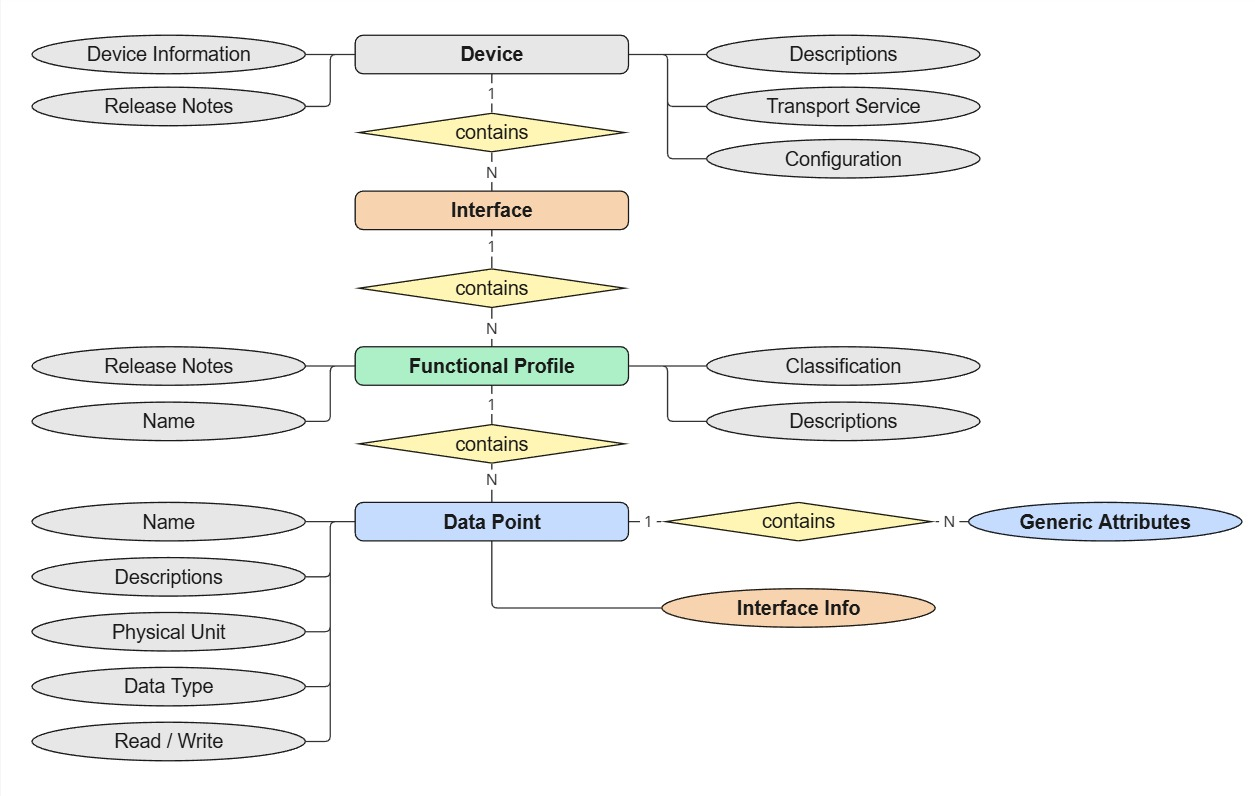
\includegraphics[width=0.7\textwidth]{ressources/product-erm.jpg}
    \caption{Entity-Relationship-Modell der Produktbeschreibung}
    \label{fig:product-erm}
\end{figure}

Ein alleinstehendes Funktionsprofil ist auf XML-Ebene durch \xmlelement{FunctionalProfileFrame} gekapselt und 
bewusst schlanker aufgebaut: Es enthält die Profil-Definition (Identifikation über Kategorie, Typ, Level of 
Operation und Version sowie Beschreibungen) und eine Liste von Datenpunkten. Diese Datenpunkte sind 
transport-neutral formuliert und beschreiben \textbf{was} eine Funktionalität anbietet, nicht \textbf{wie} sie 
technisch erreicht wird. Entsprechend enthält ein Funktionsprofil ausschliesslich generische Informationen wie 
Name, Datenrichtung, \textit{Presence Level} (Mandatory/Recommended/Optional), Datentyp, Einheit sowie textuelle 
Beschreibungen; transportspezifische Details (Register-Adressen, REST-Endpunkte, Topics, Authentisierung, etc.) 
fehlen bewusst.

\begin{figure}[H]
    \centering
    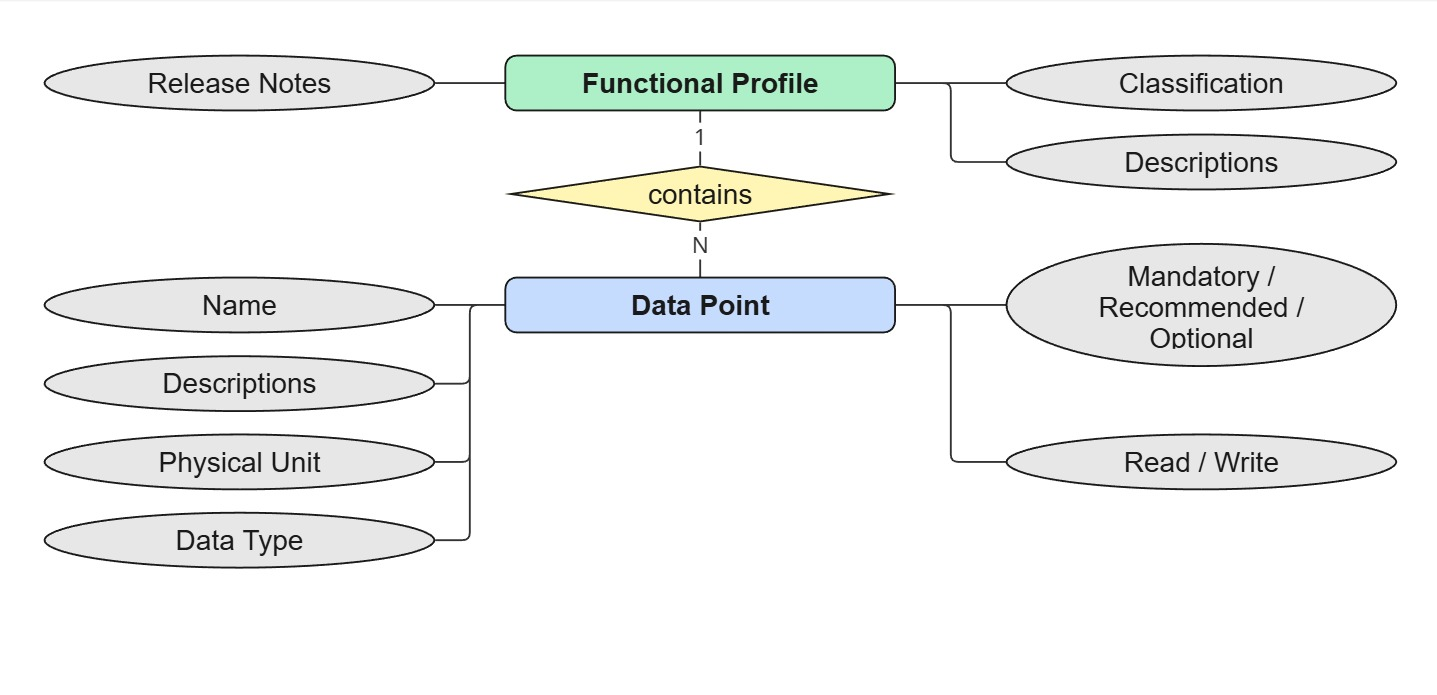
\includegraphics[width=0.7\textwidth]{ressources/functional-profile-erm.jpg}
    \caption{Entity-Relationship-Modell des Funktionsprofils}
    \label{fig:functional-profile-erm}
\end{figure}

In der Produktbeschreibung werden Funktionsprofile somit nicht als eigenständige Templates ``eingebettet'', 
sondern als protokollgebundene Instanzen konkretisiert: Die Profil-Identifikation muss passen 
(Kategorie/Typ/Level/Version) und jeder Datenpunkt wird um die zur Schnittstelle gehörenden Zugriffsinformationen 
ergänzt. Zusätzlich trägt ein Funktionsprofil im Kontext der Produktdeklaration einen Namen, um mehrere Instanzen 
im Gerät unterscheiden zu können; im alleinstehenden Funktionsprofil entfällt diese instanzbezogene Benennung.

Für Wiederverwendbarkeit bedeutet das: Nicht die gesamte alleinstehende Funktionsprofil-Deklaration ist 1:1 
wiederverwendbar, sondern die gemeinsamen, transport-neutralen Bestandteile müssen als Bausteine herausgelöst 
werden. In der Spezifikation zeigt sich diese Trennlinie u.\,a. durch \xmlelement{FunctionalProfileBase} und 
\xmlelement{DataPointBase}, die in allen Interface-Typen gleich aufgebaut sind und erst durch 
interface-spezifische Sektionen ergänzt werden. Daraus lassen sich wiederum wiederverwendbare Sektionen ableiten, 
die sowohl in Produktdeklarationen als auch in alleinstehenden Funktionsprofilen genutzt werden können 
(z.\,B. \xmlelement{alternativeNames}, \xmlelement{legibleDescriptions}, 
\xmlelement{functionalProfileIdentification}, \xmlelement{dynamicParameterList}).

\newpage

% ---------- XML-Schema Umfang ----------
\subsection{XML-Schema Umfang}

Die technische Grundlage für die SmartGridready-Deklarationen und deren Varianten ist das zugrundeliegende 
XML-Schema, dessen Umfang und Struktur die Komplexität der Implementierung massgeblich bestimmen. 
Schema-Features und Kardinalitäten geben direkt vor, welche Strukturen als korrekt gelten und wie streng ein 
Editor diese Regeln führen und validieren muss. Im Folgenden wird der Umfang zunächst anhand einiger Kennzahlen 
skizziert, danach werden zentrale XML-Schema-Features zusammengefasst und anschliessend an einem Beispiel 
illustriert. \newline

\noindent Die folgenden Kennzahlen verdeutlichen den Umfang des XML-Schemas:

\begin{itemize}
    \item 20 XSD-Dateien mit über 2'800 Zeilen Code
    \item 366 XML-Elemente, 118 komplexe Typen (\xmlelement{complexType}), 48 einfache Typen (\xmlelement{simpleType})
    \item 387 eindeutig benannte Komponenten
    \item 19 \xmlelement{choice}-Konstrukte für polymorphe Strukturen
    \item 107 Typvererbungen durch \xmlelement{extension} und \xmlelement{restriction}
    \item 636 Kardinalitäts-Definitionen, davon 41 Listen als unbounded
    \item 157 Enumerationen und Wertebereichs-Beschränkungen
\end{itemize}

% ---------- XML-Schema Features ----------
\subsubsection{XML-Schema Features}

Für die Umsetzung eines Editors bedeutet dieser Umfang nicht nur viele Felder, sondern vor allem viele 
Strukturregeln, Abhängigkeiten und Varianten, die korrekt geführt und validiert werden müssen. Die Komplexität 
des Schemas ergibt sich dabei insbesondere aus den folgenden XML-Schema-Mechanismen:
\newline


\noindent\textbf{Type Extension (Vererbung)}: \xmlelement{complexContent} mit \xmlattr{extension base} erweitert 
Basistypen wie \xmlelement{FunctionalProfileBase} und \xmlelement{DataPointBase} um interface-spezifische 
Sektionen (z.\,B. \xmlelement{restApiDataPointConfiguration}).
\newline

\noindent\textbf{Choice-Elemente (Polymorphismus)}: \xmlelement{choice} erzwingt typbasierte Varianten 
(z.\,B. in \xmlelement{InterfaceList} genau ein Interface-Typ) und führt zu unterschiedlichen Strukturen je 
nach Auswahl.
\newline

\noindent\textbf{Verschachtelte Strukturen}: Tiefe Hierarchien 
(z.\,B. \xmlelement{DeviceFrame} $\rightarrow$ \xmlelement{InterfaceList} $\rightarrow$ 
\xmlelement{FunctionalProfileList} $\rightarrow$ \xmlelement{DataPointList}) erhöhen den Aufwand für 
UI-Navigation, State und Validierung.
\newline

\noindent\textbf{Kardinalitäten und Listen}: \xmlattr{minOccurs} und \xmlattr{maxOccurs} definieren optionales 
Verhalten und Listenstrukturen (bis hin zu \xmlattr{maxOccurs="unbounded"}), die dynamisch unterstützt werden 
müssen.
\newline

\noindent\textbf{Wiederverwendung via Groups}: \xmlelement{group}-Definitionen (z.\,B. \xmlelement{DataType}) 
werden in verschiedenen Typen wiederverwendet und erhöhen die Anzahl möglicher Ausprägungen.
\newline

\noindent\textbf{Restrictions/Enumerationen}: Wertebereiche und Enumerationen definieren zulässige Werte und 
müssen im Formular sinnvoll abgebildet werden.

% ---------- XML-Schema Beispiel ----------
\subsubsection{XML-Schema Beispiel}

Abbildung~\ref{fig:xml-vs-xsd-shelly-rest} macht diese Mechanismen anhand eines realen Beispiels greifbar. Die 
Darstellung zeigt nur \textbf{kleine Ausschnitte} aus XML und XSD (vereinfacht), um die Strukturprinzipien zu 
verdeutlichen: Basistypen werden per \xmlelement{extension} erweitert, die Interface-Auswahl erfolgt über 
\xmlelement{choice}, und Listen bzw. optionale Blöcke werden durch \xmlattr{maxOccurs} und \xmlattr{minOccurs} 
gesteuert.

\begin{figure}[H]
    \centering
    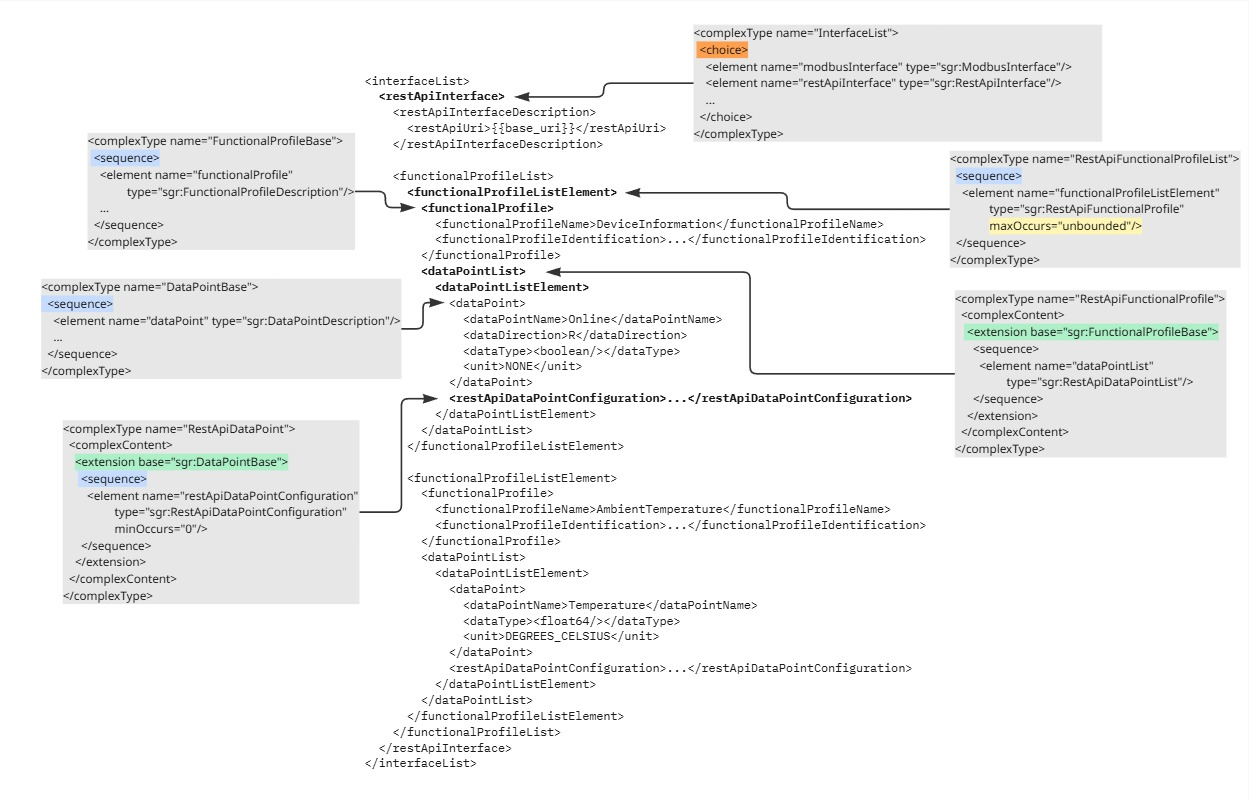
\includegraphics[width=1\textwidth]{ressources/schema-example.jpg}
    \caption{Shelly HT REST-API: Hervorgehobene Schema-Features und deren Auswirkung auf die XML-Struktur (Auszug/vereinfacht).}
    \label{fig:xml-vs-xsd-shelly-rest}
\end{figure}

Das Beispiel in Abbildung~\ref{fig:xml-vs-xsd-shelly-rest} zeigt nur einen kleinen Ausschnitt. Wie umfangreich das 
Schema tatsächlich ist, wird meist erst klar, wenn man sich darin ``einige Ebenen tief'' bewegt: Die Grundstruktur 
(Funktionsprofile und Datenpunkte) wirkt zunächst überschaubar, doch die eigentliche Komplexität entsteht durch 
viele zusätzliche Varianten und Detailbereiche, von denen die Interface-Typen nur ein Beispiel sind. Insbesondere 
REST- und Modbus-Konfigurationen können stark verschachtelt werden (z.\,B. Service-Calls mit Headern, Parametern 
und Query-Ausdrücken oder Modbus-spezifische Typvarianten, Register-/Adressierungsdetails, optionale Attribute und 
Referenzen auf Block-Reads). Gleichzeitig gibt es auch innerhalb einzelner Elemente weitere Wahlmöglichkeiten und 
optionale Unterstrukturen (z.\,B. \xmlelement{choice}-Bäume bei Datentypen, wiederverwendbare Groups, 
Enumerationen/Wertebereiche sowie teils rekursive Strukturen bei JSON-Definitionen), sodass trotz ähnlicher 
``Hülle'' sehr viele unterschiedliche, schema-konforme Ausprägungen entstehen.

In der Praxis bedeutet das für die Tool-Entwicklung: Der Editor muss Typ-Hierarchien auflösen, 
\xmlelement{choice}-Entscheidungen korrekt führen und Listen sowie optionale Sektionen dynamisch unterstützen, 
ohne dabei Schema-Konformität zu verlieren. Genau diese Kombination aus Varianten, Tiefe und Kardinalitäten prägt 
die Architektur des Deklarations-Tools und ist zugleich Grundlage für die Absicherung der Korrektheit.

% ---------- Umsetzungsansätze ----------
\subsection{Umsetzungsansätze}

Der Erfolg dieses Projekts hängt massgeblich davon ab, wie die Komplexität des XML-Schemas so kapsuliert wird, 
dass Deklarationen übersichtlich editierbar sind und gleichzeitig Schema-Regeln eingehalten werden (Siehe Fragestellung
in Abschnitt \ref{sec:fragestellungen}). In der bisherigen Analyse haben wir gelernt, wie umfangreich das XML-Schema ist 
und wie komplex die Deklarationen sein können. Damit stellt sich die Frage nach einer geeigneten Systemarchitektur und 
wie diese in einer Benutzeroberfläche abgebildet werden kann. \newline

\noindent Dazu wurden zu Projektbeginn zwei prinzipielle Implementierungsoptionen gegenübergestellt, die sich vor allem in 
der \textbf{Systemarchitektur} und der daraus ableitbaren \textbf{Benutzeroberfläche} 
unterscheiden. Folgend werden die beiden Ansätze beschrieben, Vor- und Nachteile aufgezählt und schlussendlich 
die Entscheidung erklärt.

% ---------- Ansatz 1: XML-orientierter Editor ----------
\subsubsection{Ansatz 1: XML-orientierter Editor}

Unsere erste Intuition verfolgte einen XML-zentrierten Ansatz: Die Deklaration wird dabei möglichst nahe an der 
XML-Struktur bearbeitet. Technisch wird der XML-String in ein JavaScript-Objekt konvertiert, welches der Editor 
anschliessend verarbeitet. Dabei werden Schlüsselwörter im XML-String erkannt und im UI spezifischer dargestellt: 
Beispielsweise erkennt der Editor das Element \xmlelement{legibleDescription}, extrahiert daraus das Label Legible 
Description, zeigt Regeln und Informationen (z.\,B. Kinderelemente und deren Typen) und rendert ggf. passende 
Eingabefelder (siehe Abbildung~\ref{fig:wireframe-option1}: Informationen in Blau). Der Editor würde zudem 
Listen-Elemente erkennen und indentiert darstellen; Templates stellen häufige, wiederkehrende Blöcke dar, die via 
Drag-and-Drop eingefügt werden können. Zur Validierung müsste das Tool eine Backend-Lösung bereitstellen, um die 
bereits implementierte Validierungslogik von SmartGridready einzubauen.
\begin{figure}[H]
    \centering
    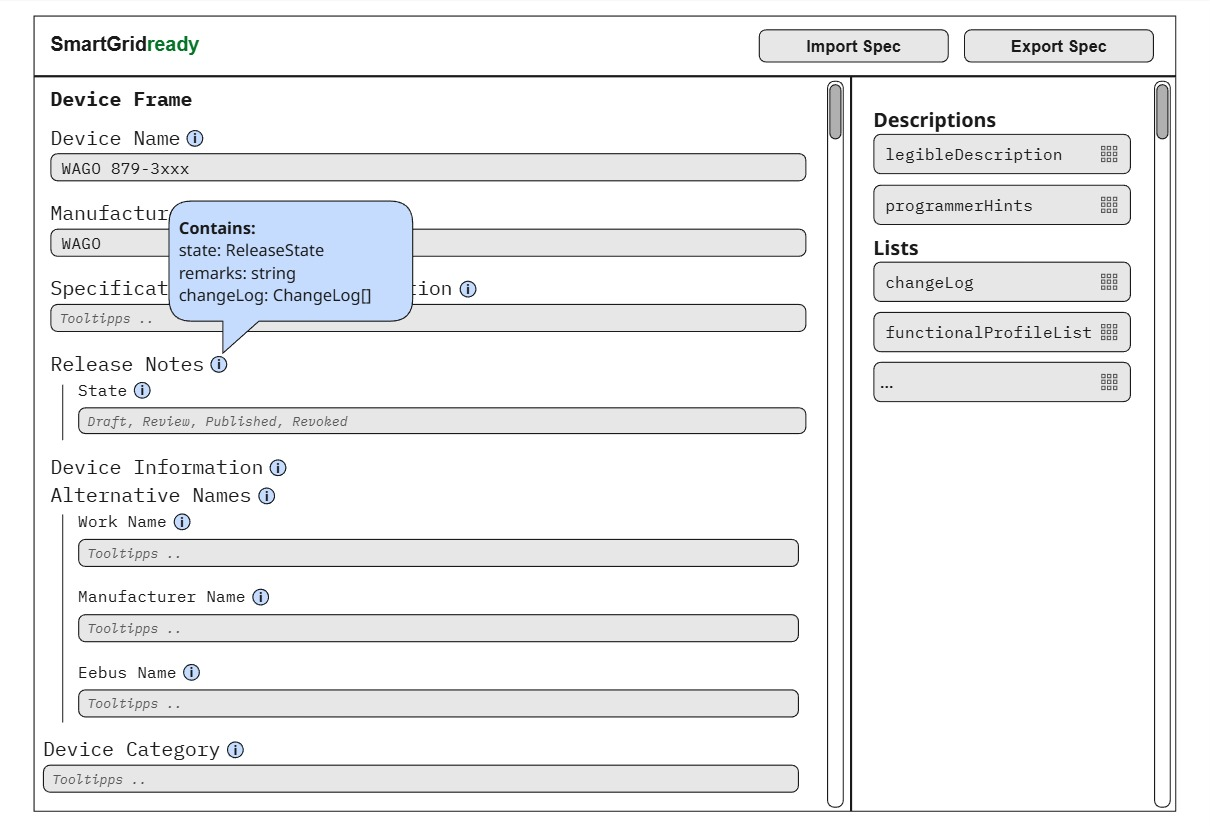
\includegraphics[width=1\textwidth]{ressources/wireframe-option1.jpg}
    \caption{Wireframe: XML-orientierter Editor.}
    \label{fig:wireframe-option1}
\end{figure}

\newpage

\noindent\textbf{Vorteile:}
\begin{itemize}
    \item Geringe Typisierungs- und Modellierungsarbeit (primär Mappings von Schlüsselwörtern und 
    UI-Darstellung).
    \item Schwächere Bindung an das XML-Schema; Schema-Änderungen lassen sich tendenziell durch zusätzliche 
    Mappings abfangen.
    \item Wiederverwendung von geprüfter SmartGridready Validierungslogik.
\end{itemize}

\noindent\textbf{Nachteile:}
\begin{itemize}
    \item Grosse Schwierigkeit, ein übersichtliches UI für verschachtelte Listen und kontextabhängige Strukturen zu 
    generieren.
    \item Der Benutzer muss dennoch Schema-Regeln beachten, um die Deklarationen korrekt zu füllen.
    \item Schema-Konformität wird erst beim Export geprüft; der Benutzer wird während der Eingabe weniger geführt.
    \item Zusätzlicher Integrations- und Betriebsaufwand durch Backend-Validierung.
\end{itemize}

% ---------- Ansatz 2: Objektmodell mit formularbasiertem UI ----------
\subsubsection{Ansatz 2: Objektmodell mit formularbasiertem UI}

Der nächste Ansatz setzt auf ein typisiertes Objektmodell als internes Datenmodell. Dazu wird das XML-Schema 
explizit in ein Typisierungsmodell überführt, welches Struktur und Kardinalitäten abbildet. Auf Basis dieses 
Modells wird dann eine Formularstruktur aufgebaut, welche die Gesamtheit der Schemaflexibilität abdeckt. 
Technisch wird der XML-String in ein JavaScript-Objekt konvertiert und anschliessend anhand des Typenmodells in 
die Formularstruktur gemappt. Der Benutzer arbeitet damit in einer geführten Maske, während das Modell gemeinsam 
mit den Formularen zulässige Strukturen vorgibt und fehlerhafte Kombinationen möglichst früh verhindert. Für den Export würde anschliessend ein Builder ebenfalls auf Basis des Typenmodells 
aus dem Objekt wieder ein konformen XML-String erzeugen. Diesen Ansatz haben wir in der Abbildung~\ref{fig:poc-option-2} 
direkt anhand unseres Proof-of-Concepts visualisiert.
\begin{figure}[H]
    \centering
    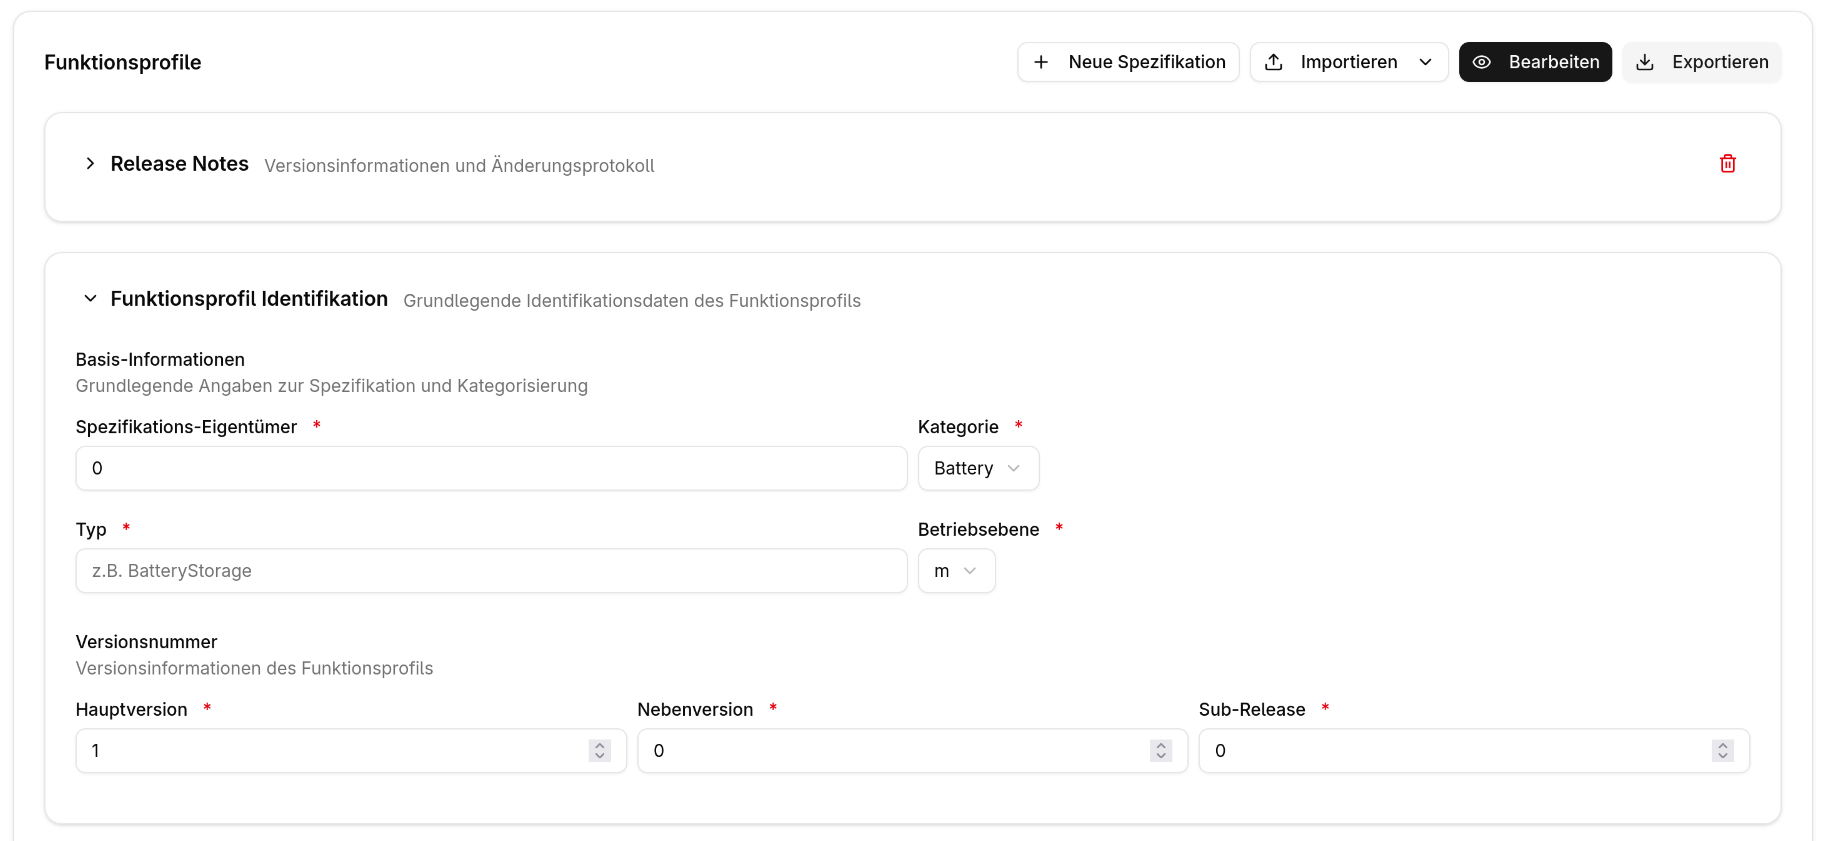
\includegraphics[width=1\textwidth]{ressources/poc-option2.png}
    \caption{POC: Erster Versuch eines formularbasiertem UI.}
    \label{fig:poc-option-2}
\end{figure}

\newpage

\noindent\textbf{Vorteile:}
\begin{itemize}
    \item Hohe Benutzerfreundlichkeit durch strukturierte, geführte Formulare. Choice-Entscheidungen, 
    Kardinalitäten und optionale Sektionen lassen sich als klare UI-Patterns abbilden.
    \item Strukturregeln können bereits während des Editierens durchgesetzt werden, statt Fehler erst beim Export 
    sichtbar zu machen.
    \item Reines Client-Side-Tool, da keine Backend-Validierung notwendig ist. Die Validierung erfolgt durch ein 
    korrektes Typenmodell und ggf. zusätzlichen Formular-Einschränkungen.
\end{itemize}

\noindent\textbf{Nachteile:}
\begin{itemize}
    \item Hoher Implementierungsaufwand (Formularaufbau, Formular Mapping / XML Building, Validierung). Diese 
    müssen jeweils die Gesamtheit vom XML-Schema decken.
    \item Schema-Änderungen müssen konsequent im Typenmodell, in den Formularen und in der Mapping/Building-Logik 
    nachgeführt werden.
\end{itemize}

% ---------- Gegenüberstellung und Entscheidung ----------
\subsubsection{Gegenüberstellung und Entscheidung}

Beim Ausprobieren von Ansatz 1 stellte sich schnell heraus, dass die Komplexität des XML-Schemas es schwierig 
macht, eine intuitive und übersichtliche Oberfläche zu erstellen. Wenn Listen mehrmals verschachtelt werden kommt 
es schnell zu Platzproblemen. Ohne eine Typisierung ist es unmöglich, die Strukturen sinnvoll zu Gruppieren. 
Zusätzlich haben wir im Abschnitt \ref{sec:smartgridready-deklarationsformate} gelernt, dass z.B. das Element 
\xmlelement{functionalProfile} nicht immer gleich definiert ist und im Produkt Kontext andere Kinder Elemente 
besitzen kann als im Funktionsprofil Kontext. Dies macht es schwierig, Informationen über die Elemente über 
Mappings zu verteilen. \newline

\noindent Entscheidend ist das Projektziel eine \textbf{intuitive, geführte Oberfläche} zu bauen, die die Komplexität des 
XML-Schemas kapselt und Schema-Regeln möglichst früh durchsetzt, statt sie nur nachgelagert zu prüfen.
Der höhere Implementierungsaufwand von Ansatz~2 ist damit eine bewusste Investition in Benutzerfreundlichkeit 
des Editors.

\newpage

\section{Konzept}
\label{sec:konzept}

Aufbauend auf der Analyse in Abschnitt~\ref{sec:analyse} stellt dieser Abschnitt das Konzept des Deklarations-Tools vor.
Es bietet eine konzeptionelle Übersicht über die Systemmodule sowie die möglichen Datenflüsse.
Die detaillierte Umsetzung folgt in Abschnitt~\ref{sec:umsetzung}.

% ---------- Systemmodule----------
\subsection{Systemmodule}

Die Systemarchitektur besteht aus mehreren Systemmodulen: \newline

\noindent\textbf{TypeScript Model:}
Das TypeScript Model ist ein aus dem XML-Schema abgeleitetes Typsystem, das die Struktur der 
SmartGridready-Deklarationen als TypeScript-Interfaces abbildet. Die Root-Typen \code{DeviceFrame} 
(für Produktbeschreibungen) und \code{FunctionalProfileFrame} (für Funktionsprofile) bilden dabei 
die Einstiegspunkte in eine hierarchische Typstruktur, die Schema-Elemente, Kardinalitäten und 
Vererbungen abbildet. Dieses Modell dient als zentrale Typdefinition für alle Systemmodule und 
gewährleistet Typensicherheit im gesamten Datenfluss. Die detaillierte Beschreibung der 
Datenmodellierung findet sich in Abschnitt~\ref{sec:datenmodellierung}.
\newline

\noindent\textbf{Mapper:}
Die Mapper konvertieren XML-Strukturen in typisierte TypeScript-Objekte, indem sie geparste 
JavaScript-Objekte in das interne Datenmodell überführen. Die Implementierung der 
Mapper wird in Abschnitt~\ref{sec:xml-parsing} beschrieben.
\newline

\noindent\textbf{Store:}
Der Store verwaltet den Editor-Zustand und persistiert Daten im Browser, sodass Inhalte beim 
Neuladen oder Schliessen erhalten bleiben. Die Umsetzung des State Management wird in 
Abschnitt~\ref{sec:state-management} erläutert.
\newline

\noindent\textbf{Editor:}
Der Editor orchestriert den Bearbeitungsworkflow und verknüpft Benutzeraktionen (Import, Export, 
Validierung, Vorschau) mit dem internen Datenmodell. Die Editor-Komponenten werden in 
Abschnitt~\ref{sec:editor-komponenten} beschrieben.
\newline

\noindent\textbf{Formulare:}
Die Formulare bilden die strukturierte Eingabemaske und ermöglichen die grafische Abbildung der 
Spezifikationselemente. Die Formular-Komponenten werden in Abschnitt~\ref{sec:formular-komponenten} 
beschrieben.
\newline

\noindent\textbf{Schemas:}
Die Schemas definieren die Validierungsregeln für die Datenstrukturen und stellen sicher, dass alle 
Schema-Regeln eingehalten werden. Die Validierung wird in Abschnitt~\ref{sec:validierung} 
detailliert beschrieben.
\newline

\noindent\textbf{Builders:}
Die Builders konvertieren die bearbeiteten TypeScript-Objekte wieder in valide XML-Deklarationen, 
indem sie das interne Datenmodell in xml2js-kompatible JavaScript-Objekte überführen und anschliessend 
in XML-Strings serialisieren. Die Implementierung der Builder wird in Abschnitt~\ref{sec:xml-building} 
beschrieben.

\newpage

% ---------- Datenfluss ----------
\subsection{Datenfluss}

Der Datenfluss beschreibt, wie eine XML-Deklaration durch das System verarbeitet wird, vom Import
bis zum Export. Abbildung~\ref{fig:concept-dataflow} visualisiert diesen Prozess und zeigt die 
Transformationen zwischen den verschiedenen Repräsentationsformen.

\begin{figure}[H]
    \centering
    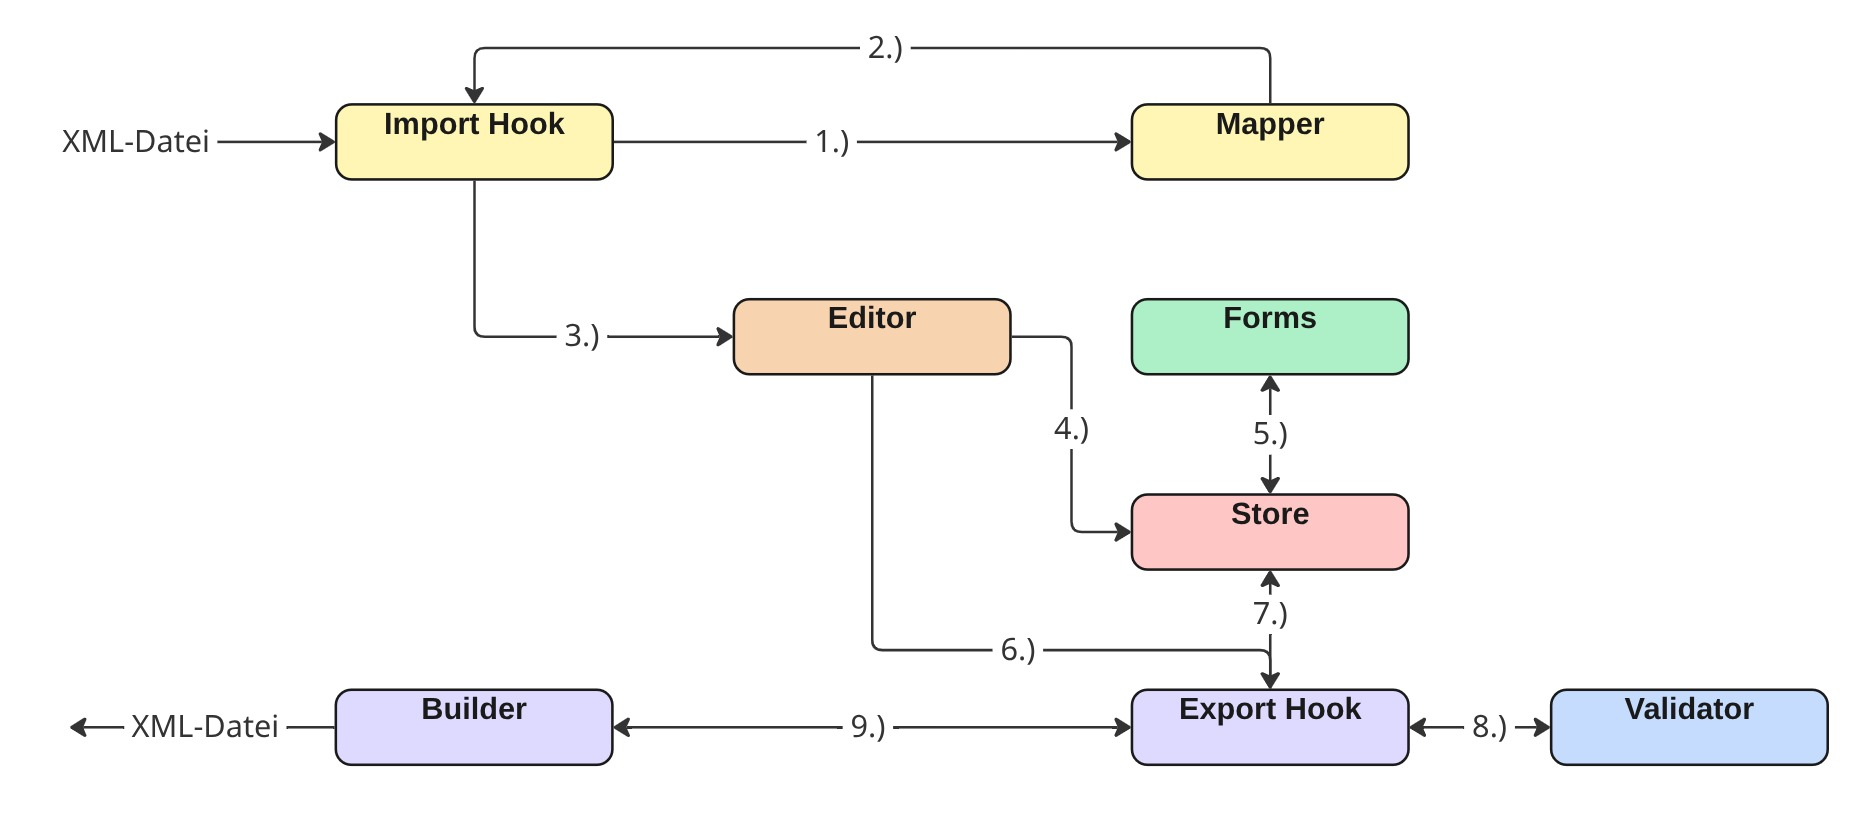
\includegraphics[width=1\textwidth]{ressources/konzept-datenfluss.jpg}
    \caption{Datenfluss des Deklarations-Tools (Konzept).}
    \label{fig:concept-dataflow}
\end{figure}

\noindent Die nummerierten Schritte im Datenfluss-Diagramm beschreiben folgende Prozesse:

\begin{enumerate}
    \item Die Import-Hook übergibt den XML-String an die Mapper-Funktionen.
    \item Die Mapper-Funktionen parsen den XML-String und konvertieren ihn in ein 
    typisiertes TypeScript-Objekt (DeviceFrame oder FunctionalProfileFrame), das sie an die 
    Import-Hook zurückgeben.
    \item Die Import-Hook benachrichtigt den Editor über den 
    erfolgreichen Import des Model-Objekts.
    \item Der Editor speichert das Model-Objekt im zentralen 
    State-Store, der den Editor-Zustand verwaltet und im Browser persistiert.
    \item Die Formular-Module lesen die Daten aus dem Store 
    und zeigen sie zur Bearbeitung an.
    \item Der Benutzer löst den Export aus, woraufhin der 
    Editor die Export-Hook aufruft.
    \item Die Export-Hook liest das aktuelle Model-Objekt 
    aus dem Store.
    \item Die Export-Hook startet die Validierung, indem 
    sie das Model-Objekt an den Validator übergibt, der es gegen das Zod-Validierungsschema prüft.
    \item Bei erfolgreicher Validierung übergibt die Export-Hook das Model-Objekt an die 
    Builder-Funktionen, die es in einen XML-String serialisieren.
\end{enumerate}

\noindent Dieser Datenfluss gewährleistet, dass Deklarationen zu jeder Zeit in einer konsistenten, typisierten 
Form vorliegen und alle Transformationen nachvollziehbar und validierbar bleiben.

\newpage

% ---------- Umsetzung des SmartGridready Deklarations-Tools ----------
\section{Umsetzung}
\label{sec:umsetzung}

Dieser Abschnitt beschreibt die technische Umsetzung des Deklarations-Tools. Es zeigt, wie die in der 
Analyse (Abschnitt~\ref{sec:analyse}) identifizierten Herausforderungen adressiert und das im Konzept 
(Abschnitt~\ref{sec:konzept}) entworfene System realisiert wurde.

\subsection{Technologie-Stack}

Das Tool basiert auf einem modernen Web-Stack, der sich durch breiten Community-Support und ein 
ausgereiftes Ökosystem auszeichnet. \newline

\noindent\textbf{React mit Next.js} bildet die Basis für eine komponentenorientierte Entwicklung. React ermöglicht 
es, wiederkehrende Schema-Sektionen als wiederverwendbare Komponenten zu implementieren. Next.js bietet dabei 
eine robuste Projektstruktur mit integriertem Routing. \newline

\noindent\textbf{TypeScript} gewährleistet Typsicherheit bei komplexen, verschachtelten Datenstrukturen. Fehler 
werden bereits zur Entwicklungszeit sichtbar, was besonders bei der Mapping-Logik und der Weitergabe von Daten 
zwischen Editor, Validierung und Export hilfreich ist. \newline

\noindent\textbf{xml2js} übernimmt das XML-Parsing beim Import und die Serialisierung beim Export. Die Bibliothek 
wandelt XML in JavaScript-Objekte um und umgekehrt, sodass bestehende Deklarationen geladen, bearbeitet und als 
gültige XML-Datei ausgegeben werden können. \newline

\noindent\textbf{Zustand} verwaltet den Editor-Zustand leichtgewichtig und ohne Boilerplate. Mit der 
Persist-Middleware wird der Bearbeitungsstand automatisch im Browser gespeichert, sodass Inhalte bei Neuladen 
erhalten bleiben. \newline

\noindent\textbf{Zod} ergänzt TypeScript um Laufzeit-Validierung. Constraints wie String-Längen oder 
Array-Obergrenzen, die das Typsystem nicht abbilden kann, werden damit zur Laufzeit geprüft und als 
Fehlermeldungen in der Oberfläche angezeigt. \newline

\noindent\textbf{Shadcn/UI mit Tailwind CSS} liefert konsistente, zugängliche UI-Komponenten für Formulare, 
Dialoge und Navigation. \newline  

\newpage

% ---------- Sektionbasierte Dateistruktur ----------
\subsection{Sektionsbasierte Dateistruktur}
\label{sec:sektionsbasierte-dateistruktur}

Ein zentrales Architekturprinzip ist die \textbf{sektionsbasierte Organisation} des Source-Codes. Die 
Ordner- und Dateistruktur ist dem XML-Schema angelehnt: Bereiche wie \textit{DeviceInformation}, 
\textit{InterfaceList} oder \textit{FunctionalProfile} erhalten jeweils einen eigenen Ordner mit 
spezifischen Dateien für Formular (UI-Komponente), Mapper (XML $\rightarrow$ Model), Builder 
(Model $\rightarrow$ XML), Schema (Zod-Validierung) und Store-Slice (State-Actions). Der 
\textit{shared}-Ordner enthält wiederverwendbare Komponenten, die von mehreren 
Sektionen genutzt werden.

\begin{figure}[H]
    \centering
    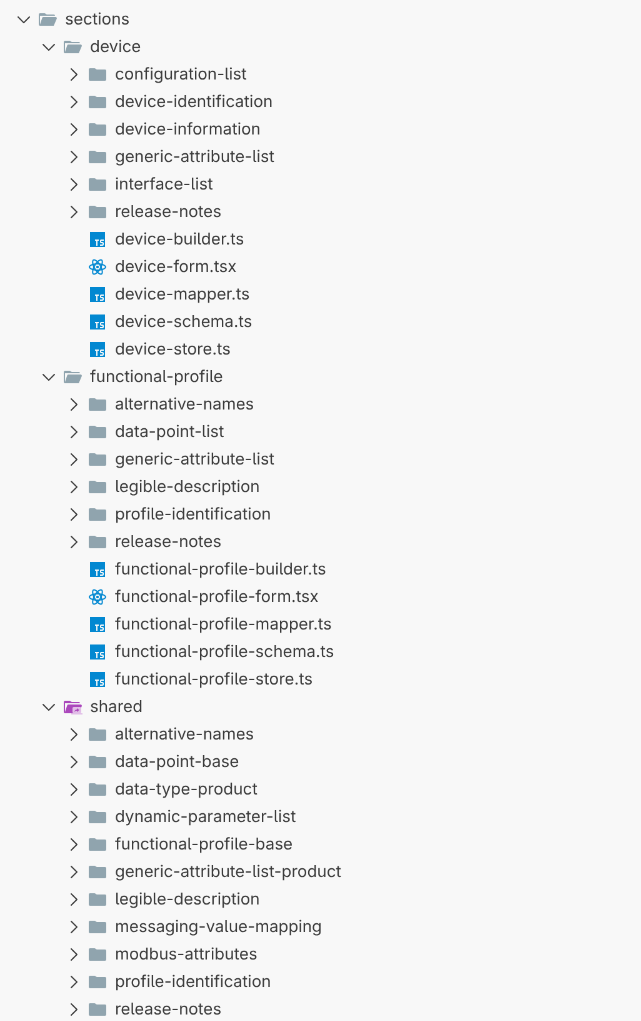
\includegraphics[width=0.6\textwidth]{ressources/file-structure.png}
    \caption{Sektionsbasierte Dateistruktur.}
    \label{fig:file-structure}
\end{figure}

\noindent Der Vorteil dieser Organisation: Bei Änderungen am XML-Schema sind nur die betroffenen Sektionen 
anzupassen. Fügt SmartGridready beispielsweise ein neues Attribut zu \textit{DeviceInformation} 
hinzu, müssen nur die entsprechende Stelle im TypeScript-Modell und die Dateien im jeweiligen 
Sektions-Ordner erweitert werden -- der Rest der Codebasis bleibt unberührt. Diese Modularität 
erleichtert auch die Einarbeitung: Entwickler können eine Sektion verstehen, ohne die gesamten Codebase 
überblicken zu müssen. \newline

\newpage

% ---------- TypeScript Model ----------
\subsection{Datenmodellierung}
\label{sec:datenmodellierung}

Die Datenmodellierung adressiert zu einem Teil die Fragestellung, wie die \textbf{Korrektheit der Struktur und Inhalte} 
sichergestellt werden kann (siehe Abschnitt~\ref{sec:fragestellungen}). Um diese Struktur vom XML-Schema im 
TypeScript-Code abzubilden, wurde ein typisiertes Datenmodell entwickelt, das die Schema-Hierarchie, Kardinalitäten und 
Datentypen in Interfaces und Types übersetzt. Dies ermöglicht eine durchgängige Typsicherheit im gesamten Quellcode.

\subsubsection{Ableitung aus dem XML-Schema}

Die Übersetzung erfolgte manuell durch systematische Analyse der XSD-Dateien. Dabei wurden folgende 
Mapping-Regeln angewandt:
\begin{itemize}[noitemsep,topsep=0pt]
    \item \xmlelement{complexType} $\rightarrow$ TypeScript-Interface
    \item \xmlelement{simpleType}/Enumerationen $\rightarrow$ Union-Types oder String-Literal-Types
    \item \xmlelement{extension} (Vererbung) $\rightarrow$ Interface-Extension
    \item \xmlelement{choice} $\rightarrow$ Optionale Properties oder Union-Types
\end{itemize}

\noindent Kardinalitäten werden direkt übernommen: \xmlattr{minOccurs="0"} wird zu optionalen Properties (\code{?}), 
\xmlattr{maxOccurs="unbounded"} zu Arrays. Feste Obergrenzen wie \xmlattr{maxOccurs="4"} lassen sich im 
Typsystem nicht ausdrücken und werden über die Validierung sichergestellt (Abschnitt~\ref{sec:validierung}).

\noindent Abbildung~\ref{fig:xsd-functional-profile} und \ref{fig:ts-functional-profile} zeigen diese Übersetzung 
am Beispiel FunctionalProfileBase und FunctionalProfileDescription.

\begin{figure}[H]
    \centering
    \begin{lstlisting}[language=xsdselective,frame=single,backgroundcolor=\color{gray!10},basicstyle=\ttfamily\scriptsize,breaklines=true]
  <complexType name="FunctionalProfileBase">
    <sequence>
      <element name="functionalProfile" type="sgr:FunctionalProfileDescription" />
      <element name="genericAttributeList" 
               type="sgr:GenericAttributeListProduct" minOccurs="0" />
    </sequence>
  </complexType>
  <complexType name="FunctionalProfileDescription">
    <sequence>
      <element name="functionalProfileName" type="string" />
      <element name="functionalProfileIdentification" type="sgr:FunctionalProfileIdentification" />
      <element name="alternativeNames" type="sgr:AlternativeNames" minOccurs="0" />
      <element name="legibleDescription" type="sgr:LegibleDescription" 
               maxOccurs="4" minOccurs="0" />
      <element name="programmerHints" type="sgr:LegibleDescription" 
               maxOccurs="4" minOccurs="0" />
    </sequence>
  </complexType>
    \end{lstlisting}
    \caption{XML-Schema: FunctionalProfileBase und FunctionalProfileDescription}
    \label{fig:xsd-functional-profile}
\end{figure}

\begin{figure}[H]
    \centering
    \begin{lstlisting}[language=typescriptselective,frame=single,backgroundcolor=\color{gray!10},basicstyle=\ttfamily\scriptsize,breaklines=true]
export interface FunctionalProfileBase {
  functionalProfile: FunctionalProfileDescription;
  genericAttributeList?: GenericAttributeListProduct;
}

export interface FunctionalProfileDescription {
  functionalProfileName: string;
  functionalProfileIdentification: FunctionalProfileIdentification;
  alternativeNames?: AlternativeNames;
  legibleDescription?: LegibleDescription[]; // maxOccurs="4"
  programmerHints?: LegibleDescription[]; // maxOccurs="4"
}
    \end{lstlisting}
    \caption{TypeScript-Datenmodell: FunctionalProfileBase und FunctionalProfileDescription}
    \label{fig:ts-functional-profile}
\end{figure}

\noindent Pflichtfelder bleiben required, optionale Elemente (\xmlattr{minOccurs="0"}) werden zu \code{?}-Properties, 
und Arrays dokumentieren die Obergrenze als Kommentar.

\newpage
% ---------- Mapper ----------
\subsection{Mapper}
\label{sec:xml-parsing}

Der Mapper transformiert importierte XML-Deklarationen in typisierte Model-Objekte. Beim Import einer 
bestehenden Deklaration über Datei-Upload oder aus der SGr-Library wird der XML-String zunächst 
geparst und anschliessend in die interne Datenstruktur überführt. 

\subsubsection{Prozess}
Abbildung~\ref{fig:mapper-prozessablauf} 
zeigt den Ablauf: Eine Parser-Funktion liest den XML-String, wandelt ihn via xml2js in ein
JavaScript-Objekt um und delegiert dieses an hierarchisch organisierte Mapper-Funktionen.

\begin{figure}[H]
    \centering
    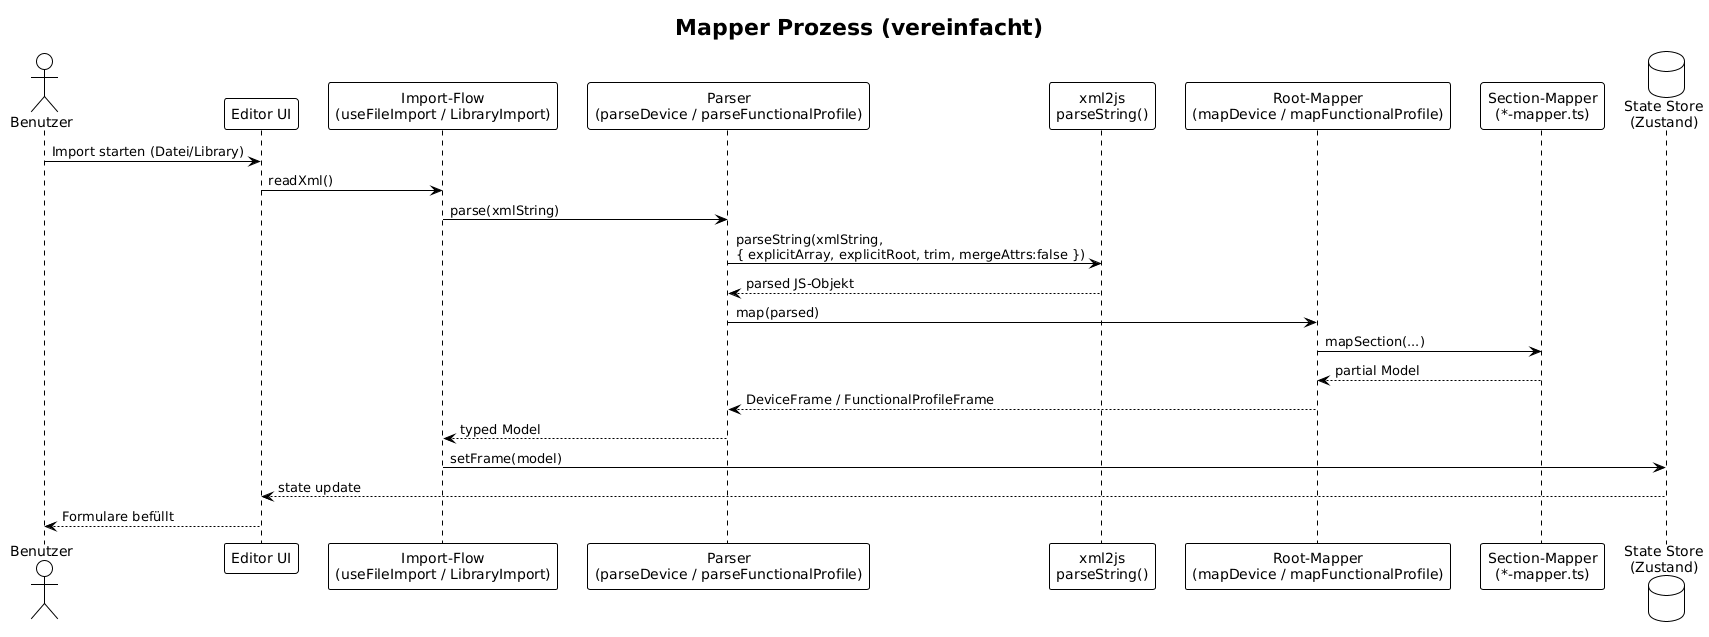
\includegraphics[width=1\textwidth]{ressources/sequenz-diagramm-mapper.png}
    \caption{Sequenzdiagramm: Mapper-Prozess (vereinfacht)}
    \label{fig:mapper-prozessablauf}
\end{figure}

\subsubsection{xml2js-Konfiguration}

Im ersten Schritt parst xml2js den XML-String. Die Konfiguration bestimmt, wie die 
XML-Struktur in ein JavaScript-Objekt übersetzt wird:
\begin{itemize}[noitemsep,topsep=0pt]
    \item \code{explicitArray: true} -- Jedes Element wird als Array behandelt, auch wenn es nur einmal 
          vorkommt. Dies ermöglicht einheitlichen Zugriff ohne Fallunterscheidung.
    \item \code{mergeAttrs: false} -- XML-Attribute werden unter \code{\$} gruppiert, anstatt mit 
          Kindelementen vermischt zu werden.
    \item \code{explicitRoot: true} -- Das Root-Element bleibt erhalten, was die Navigation erleichtert.
    \item \code{trim: true} -- Whitespace um Textinhalte wird entfernt.
\end{itemize}

\noindent Abbildung~\ref{fig:xml2js-mapper} zeigt die Parser-Funktion \code{parseDevice}. Nach dem 
Parsen wird das JavaScript-Objekt an \code{mapDevice} übergeben.

\begin{figure}[H]
    \centering
    \begin{lstlisting}[language=typescriptselective,frame=single,backgroundcolor=\color{gray!10},basicstyle=\ttfamily\scriptsize,breaklines=true]
export async function parseDevice(xmlString: string): Promise<DeviceFrame> {
  let parsed: any;
  try {
    parsed = await new Promise<any>((resolve, reject) => {
      parseString(
        xmlString,
        { explicitArray: true, mergeAttrs: false, explicitRoot: true, trim: true },
        (err, result) => 
          if (err) reject(err);
          else resolve(result);
      );
    });
  } catch (error) { // Handle error }
  return mapDevice(parsed);
}
    \end{lstlisting}
    \caption{TypeScript-Code: parseDevice Funktion (vereinfacht)}
    \label{fig:xml2js-mapper}
\end{figure}

\newpage

\subsubsection{Mapper-Hierarchie}

Das geparste JavaScript-Objekt wird nun von hierarchisch organisierten Mappern verarbeitet. Der 
Root-Mapper \code{mapDevice} (Abbildung~\ref{fig:mapper-hierarchy}) extrahiert das Root-Element 
und delegiert an Section-Mapper. Jeder Section-Mapper gibt ein typisiertes Teilobjekt zurück, das 
dem entsprechenden TypeScript-Interface entspricht.

\begin{figure}[H]
    \centering
    \begin{lstlisting}[language=typescriptselective,frame=single,backgroundcolor=\color{gray!10},basicstyle=\ttfamily\scriptsize,breaklines=true]
// device-mapper.ts - Root-Mapper
function mapDevice(parsed: ParsedDeviceXml): DeviceFrame {
  const frameData = parsed.DeviceFrame;
  
  // Section-Mapper aufrufen und typisiertes Objekt zusammenbauen
  const device: DeviceFrame = {
    ...mapDeviceIdentification(frameData),
    releaseNotes: mapReleaseNotes(getFirstElement(frameData, "releaseNotes")),
    deviceInformation: mapDeviceInformation(getFirstElement(frameData, "deviceInformation")),
    interfaceList: mapInterfaceList(getFirstElement(frameData, "interfaceList")),
  };
  
  return device;
}
    \end{lstlisting}
    \caption{Root-Mapper: Delegation an Section-Mapper}
    \label{fig:mapper-hierarchy}
\end{figure}

\noindent Die Section-Mapper extrahieren die Werte aus dem geparsten Objekt und weisen sie den 
Properties des TypeScript-Interfaces zu (Abbildung~\ref{fig:section-mapper}). Das Ergebnis ist 
ein vollständig typisiertes Model-Objekt, das in den Store geschrieben werden kann.

\begin{figure}[H]
    \centering
    \begin{lstlisting}[language=typescriptselective,frame=single,backgroundcolor=\color{gray!10},basicstyle=\ttfamily\scriptsize,breaklines=true]
// device-information-mapper.ts - Section-Mapper
export function mapDeviceInformation(xml: Xml2JsObject): DeviceInformation {
  const deviceInformation: DeviceInformation = {
    // Pflichtfelder direkt extrahieren
    deviceCategory: getTypedValue<DeviceCategory>(xml, "deviceCategory", "SubMeterElectricity"),
    isLocalControl: getStringValue(xml, "isLocalControl") === "true",
  };

  // Optionale Felder nur setzen wenn vorhanden
  setOptionalField(deviceInformation, "brandName", getOptionalStringValue(xml, "brandName"));
  setOptionalField(deviceInformation, "softwareRevision", getOptionalStringValue(xml, "softwareRevision"));
  // ... weitere optionale Felder

  return deviceInformation;
}
    \end{lstlisting}
    \caption{Section-Mapper: Extraktion und Zuweisung an Interface-Properties}
    \label{fig:section-mapper}
\end{figure}

\newpage

% ---------- Store ----------
\subsection{State Management}
\label{sec:state-management}

Nach dem Mapping wird das typisierte Model-Objekt im zentralen State Store gespeichert. Dieser Store ist 
die Single Source of Truth während der Bearbeitung: Alle Formular-Komponenten lesen daraus, alle Eingaben 
schreiben hinein, und beim Export wird er zur XML-Generierung verwendet.

Für das State Management wurde \textbf{Zustand} gewählt, eine leichtgewichtige Alternative zu Redux. Zustand 
verzichtet auf Boilerplate wie Actions und Reducers -- State und Actions werden direkt in einem Objekt 
definiert. Die Architektur umfasst drei getrennte Stores: \code{DeviceStore} für Produktbeschreibungen, 
\code{ProfileStore} für Funktionsprofile und einen \code{ValidationStore} für den globalen Validierungszustand.

\subsubsection{Slice-Architektur}

Die Stores sind modular in \textbf{Slices} organisiert. Ein Slice kapselt alle Actions für einen bestimmten 
Bereich des State-Objekts. Diese Struktur spiegelt die sektionsbasierte Architektur wider: Der 
\code{DeviceInformationSlice} enthält beispielsweise \code{updateDeviceCategory()}, \code{updateBrandName()} 
und weitere Actions, die ausschliesslich den \code{deviceInformation}-Block betreffen.

Slices können hierarchisch komponiert werden: Der \code{InterfaceListSlice} bindet für jede Schnittstelle 
wiederum den \code{FunctionalProfileListSlice} ein, welcher seinerseits den \code{DataPointListSlice} 
enthält. Diese Komposition ermöglicht es, die tiefe Verschachtelung des XML-Schemas abzubilden, während 
jede Ebene isoliert testbar bleibt. Abbildung~\ref{fig:device-store} zeigt die Store-Konfiguration mit den 
eingebundenen Slices.

\begin{figure}[H]
    \centering
    \begin{lstlisting}[language=typescriptselective,frame=single,backgroundcolor=\color{gray!10},basicstyle=\ttfamily\scriptsize,breaklines=true]
export const useDeviceStore = create<DeviceStoreState>()(
  persist(
    immer((set) => ({
      device: undefined,

      setDevice: (device) =>
        set((state) => {
          state.device = device;
        }),

      createEmpty: () =>
        set((state) => {
          state.device = createEmptyDevice();
        }),

      clear: () =>
        set((state) => {
          state.device = undefined;
        }),

      ...createDeviceIdentificationSlice(set),
      ...createReleaseNotesSliceForDevice(set),
      ...createDeviceInformationSlice(set),
      ...createConfigurationListSlice(set),
      ...createGenericAttributeListSlice(set),
      ...createInterfaceListSlice(set),
    })),
    {
      name: "sgr-device-storage",
      storage: debouncedStorage<DeviceStoreState>(),
      partialize: (state) => ({ device: state.device }) as DeviceStoreState,
    }
  )
);
    \end{lstlisting}
    \caption{TypeScript-Code: DeviceStore mit Middleware-Stack und Slice-Komposition}
    \label{fig:device-store}
\end{figure}

\subsubsection{Middleware-Stack}

Der Store verwendet zwei Middlewares, die ineinander verschachtelt werden, \code{immer} und \code{persist} 
(siehe Abbildung~\ref{fig:device-store}). \newline

\noindent Die \textbf{Immer Middleware} ermöglicht immutable State-Updates mit mutabler Syntax. Ohne Immer müssten 
verschachtelte Updates wie: \newline \code{device.interfaceList[0].functionalProfileList[2].dataPointList[1].name} 
auf jeder Ebene kopiert werden. Mit Immer kann stattdessen direkt auf die Property geschrieben werden -- 
die Middleware erzeugt automatisch eine neue, immutable Kopie des State (Abbildung~\ref{fig:immer-action}). \newline

\begin{figure}[H]
  \centering
  \begin{lstlisting}[language=typescriptselective,frame=single,backgroundcolor=\color{gray!10},basicstyle=\ttfamily\scriptsize,breaklines=true]
updateDeviceName: (value) =>
set((state) => {
  const device = getDevice(state);
  if (device) device.deviceName = value;  // Mutable Syntax, immutable Update
}),
  \end{lstlisting}
  \caption{Slice-Action mit Immer: Mutable Syntax, immutables Update}
  \label{fig:immer-action}
\end{figure}

\noindent Die \textbf{Persist Middleware} speichert den State automatisch im localStorage. Bei jedem 
State-Update wird der aktuelle Zustand serialisiert und gespeichert. Beim Neuladen der Seite wird er 
wiederhergestellt, sodass der Bearbeitungsstand erhalten bleibt.

\subsubsection{Debounced Storage}

Ein Performance-Problem der Standard-Persist-Middleware: Jeder Tastendruck löst ein State-Update und damit 
einen synchronen \code{localStorage.setItem()}-Aufruf aus. Bei schnellem Tippen führt dies zu spürbaren 
Verzögerungen, da der Hauptthread blockiert wird. \newline

\noindent Die Lösung ist ein \textbf{Debounced Storage Adapter} (Abbildung~\ref{fig:debounced-storage}). Statt sofort 
zu schreiben, startet er einen Timer. Kommt innerhalb von 1000\,ms ein weiteres Update, wird der Timer 
zurückgesetzt. Erst wenn eine Sekunde ohne Änderungen verstreicht, wird der finale Zustand tatsächlich 
persistiert. Bei schnellem Tippen wird so nur ein einziger Schreibvorgang ausgeführt.

\begin{figure}[H]
    \centering
    \begin{lstlisting}[language=typescriptselective,frame=single,backgroundcolor=\color{gray!10},basicstyle=\ttfamily\scriptsize,breaklines=true]
export function createDebouncedStorage<T>(delayMs: number = 1000): PersistStorage<T> {
  const timeouts = new Map<string, NodeJS.Timeout>();

  return createJSONStorage<T>(() => ({
    getItem: (name) => localStorage.getItem(name),

    setItem: (name, value) => {
      // Vorherigen Timeout abbrechen (falls vorhanden)
      if (timeouts.has(name)) clearTimeout(timeouts.get(name));

      // Neuen Timeout setzen: Schreiben erst nach delayMs Inaktivitaet
      timeouts.set(name, setTimeout(() => {
        localStorage.setItem(name, value);
        timeouts.delete(name);
      }, delayMs));
    },

    removeItem: (name) => localStorage.removeItem(name),
  })) as PersistStorage<T>;
}
    \end{lstlisting}
    \caption{TypeScript-Code: Debounced Storage Adapter für Zustand Persist (vereinfacht)}
    \label{fig:debounced-storage}
\end{figure}

\noindent Mögliche Verbesserungen wie Store-Splitting werden in Abschnitt~\ref{sec:future-work} beschrieben.

\newpage

% ---------- Editor ----------
\subsection{Editor}
\label{sec:editor-komponenten}

Der Editor bildet die zentrale Benutzeroberfläche des Tools. Er orchestriert den kompletten Bearbeitungsworkflow: 
Import bestehender Deklarationen, Bearbeitung über Formulare, Vorschau der generierten XML-Struktur und 
Export als valide XML-Datei.

\subsubsection{Komponenten-Architektur}

Die Architektur trennt Container- von Präsentationslogik (Abbildung~\ref{fig:editor-architektur}). Der 
\code{EditorContainer} ist eine wiederverwendbare Komponente, die deklarationsunabhängige Funktionalität 
kapselt: Header mit Titel und Aktions-Buttons, Import-Dialog, Vorschau-Panel und Toast-Benachrichtigungen.

Die spezifischen Editoren (\code{DeviceEditor}, \code{FunctionalProfileEditor}) werden als Kinder 
eingebettet und erhalten ihre Konfiguration über Props: welcher Builder und Validator verwendet wird, 
welche Formulare angezeigt werden und woher die Library-Daten stammen. Diese Trennung ermöglicht es, 
neue Deklarationstypen (z.\,B. für Communicators) mit minimalem Aufwand hinzuzufügen.

\begin{figure}[H]
    \centering
    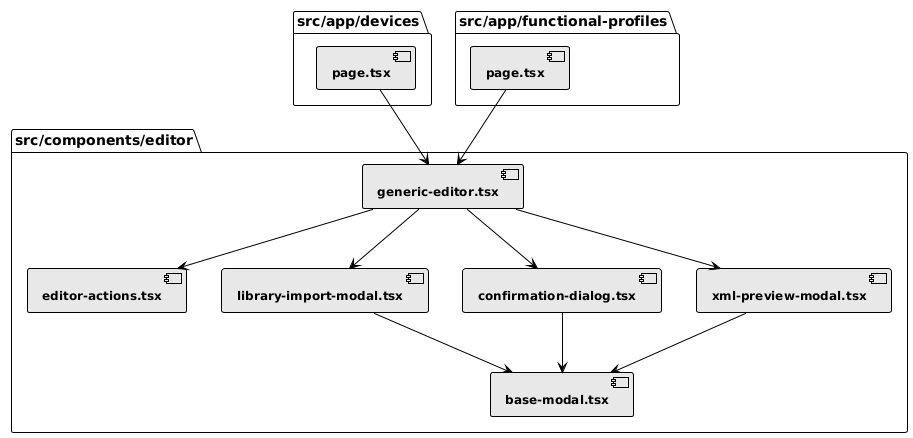
\includegraphics[width=1\textwidth]{ressources/editor-komponenten-architektur.png}
    \caption{Architektur der Editor-Komponenten}
    \label{fig:editor-architektur}
\end{figure}

\subsubsection{XSLT-Vorschau}
\label{sec:xslt-vorschau}

Während der Bearbeitung können Nutzer jederzeit eine formatierte Vorschau der Deklaration aufrufen. Diese 
zeigt, wie das generierte XML aussehen wird -- nicht als Rohtext, sondern als strukturierte HTML-Ansicht mit 
Überschriften, Tabellen und Formatierungen. \newline  

\noindent Die \textbf{XSL-Stylesheets wurden von SmartGridready bereitgestellt}. Diese definieren, wie die verschiedenen 
XML-Elemente visuell dargestellt werden: Farben, Layouts und welche Informationen hervorgehoben werden. Die 
Stylesheets sind modular aufgebaut (\code{DeviceFrame.xsl}, \code{FunctionalProfile.xsl}, etc.) und 
referenzieren sich gegenseitig über \code{xsl:include}. \newline

\noindent Eine technische Herausforderung: Der Browser-native \code{XSLTProcessor} löst \code{xsl:include}-Referenzen 
nicht automatisch über das Netzwerk auf. Die Lösung ist eine rekursive Vorverarbeitung, die alle referenzierten 
Stylesheets lädt und inline einbettet, bevor die Transformation ausgeführt wird.

\newpage

% ---------- Forms ----------
\subsection{Formular-Komponenten}
\label{sec:formular-komponenten}

Die Formular-Komponenten adressieren die Fragestellung, wie die \textbf{Elemente der Spezifikation graphisch 
abgebildet} werden können (siehe Abschnitt~\ref{sec:fragestellungen}). Ziel ist es, die abstrakte XML-Struktur 
in eine intuitive Eingabemaske zu übersetzen, die keine XML-Kenntnisse voraussetzt. \newline  

\noindent Der Aufbau orientiert sich an der Schema-Hierarchie (Abbildung~\ref{fig:ui-editor-overview}): Aufklappbare 
\textbf{FormSections} repräsentieren Schema-Blöcke wie \textit{Device Information} oder 
\textit{Interface List}. FormSections können verschachtelt werden, um die hierarchische Struktur des Schemas 
abzubilden -- etwa eine \textit{Functional Profile}-Section innerhalb einer \textit{Interface}-Section. 
\textbf{FormGroups} gruppieren thematisch zusammengehörige Felder innerhalb einer Section. \newline

\noindent Die Schema-Kardinalitäten werden visuell kommuniziert: Pflichtfelder (\xmlattr{minOccurs="1"}) sind durch ein 
Sternchen gekennzeichnet, wiederholbare Elemente (\xmlattr{maxOccurs="unbounded"}) erscheinen als dynamische 
Listen mit Add- und Remove-Buttons. \newline

\begin{figure}[H]
    \centering
    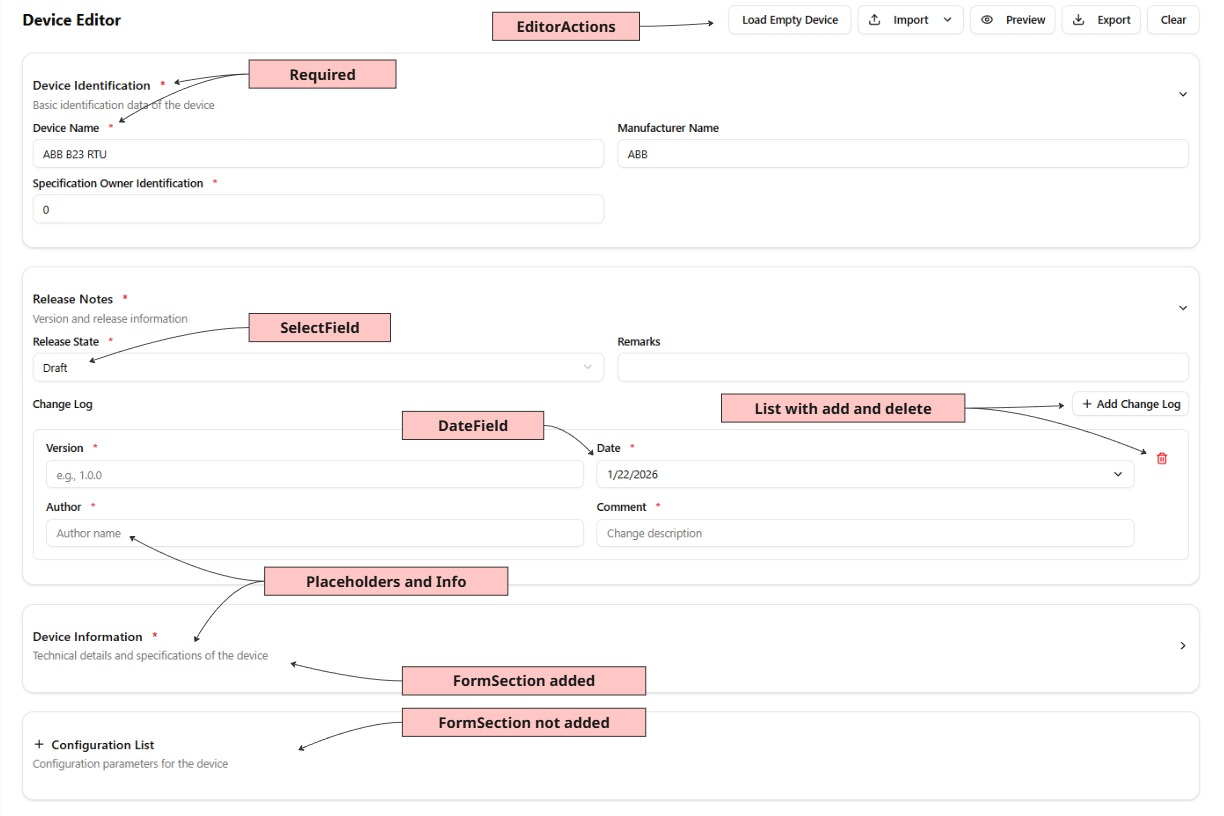
\includegraphics[width=1\textwidth]{ressources/editor-ui.jpg}
    \caption{UI-Übersicht der Formular-Komponenten}
    \label{fig:ui-editor-overview}
\end{figure}

\newpage

\noindent Die Formularstrukturen werden \textbf{deklarativ} über Props zusammengestellt 
(Abbildung~\ref{fig:form-section-code}). Entwickler spezifizieren, welche Felder angezeigt werden, ob sie 
Pflichtfelder sind und woher die Daten kommen -- Layout, Styling und Interaktionslogik werden von den 
Basiskomponenten konsistent bereitgestellt. Das Feld \code{error} bindet dabei an die Validierung: Ist \newline
\code{validationAttempted} gesetzt und existiert ein Fehler für dieses Feld, wird die Fehlermeldung 
angezeigt (siehe Abschnitt~\ref{sec:validierung}).

\begin{figure}[H]
    \centering
    \begin{lstlisting}[language=jsxselective,frame=single,backgroundcolor=\color{gray!10},basicstyle=\ttfamily\scriptsize,breaklines=true]
      <FormSection title="Device Identification" description="Basic identification data of the device" required={true}>
        <FormGroup>
          <InputField
            label="Device Name"
            name="deviceName"
            required={true}
            type="text"
            value={deviceName ?? ""}
            onChange={(value) => store.updateDeviceName(value)}
            error={getError("deviceName")}
          />
          <InputField
            label="Manufacturer Name"
            name="manufacturerName"
            required={false}
            type="text"
            value={manufacturerName ?? ""}
            onChange={(value) => store.updateManufacturerName(value || undefined)}
            error={getError("manufacturerName")}
          />
        </FormGroup>

        <FormGroup>
          <InputField
            label="Specification Owner Identification"
            name="specificationOwnerIdentification"
            required={true}
            type="text"
            value={specificationOwnerIdentification ?? ""}
            onChange={(value) => store.updateSpecificationOwnerIdentification(value)}
            error={getError("specificationOwnerIdentification")}
          />
        </FormGroup>
    </FormSection>
    \end{lstlisting}
    \caption{Deklarative Formular-Definition (vereinfacht)}
    \label{fig:form-section-code}
\end{figure}

\noindent Der Code gezeigt in Abbildung \ref{fig:form-section-code} leitet folgendes UI ab in Abbildung \ref{fig:form-section-ui}

\begin{figure}[H]
  \centering
  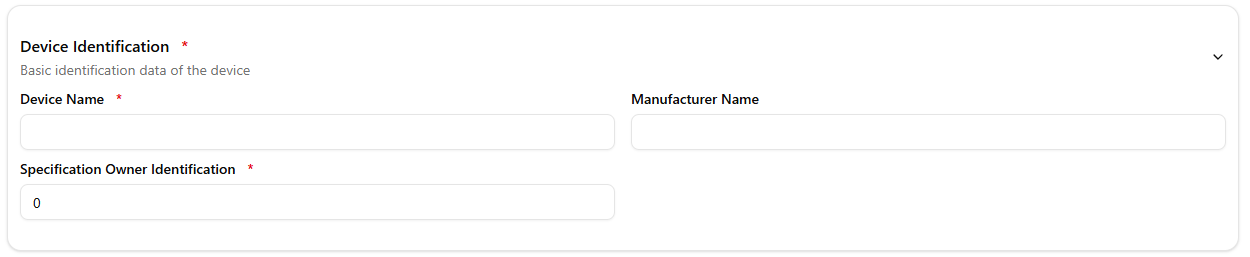
\includegraphics[width=1\textwidth]{ressources/device-identification.png}
  \caption{Device Identification UI}
  \label{fig:form-section-ui}
\end{figure}

\newpage

% ---------- Validierung ----------
\subsection{Validierung}
\label{sec:validierung}

Die Validierung schliesst die Fragestellung nach der \textbf{Korrektheit der Inhalte}  ab
(Abschnitt~\ref{sec:fragestellungen}). Während das TypeScript-Datenmodell strukturelle Typsicherheit 
zur Compile-Zeit bietet, kann es bestimmte Constraints nicht ausdrücken: String-Längen, Zahlenbereiche 
oder Array-Obergrenzen. Diese werden durch Laufzeit-Validierung mit Zod ergänzt.

\subsubsection{Prozess}

Die Validierung wird ausgelöst, wenn der Nutzer einen Export startet (Abbildung~\ref{fig:validation-flow}). 
Der Export-Hook ruft das Zod-Schema auf und setzt anschliessend \code{validationAttempted = true} im 
\code{ValidationStore} -- unabhängig davon, ob Fehler gefunden wurden. Dieses Flag steuert, ob 
Formular-Komponenten ihre Fehler anzeigen: Vor dem ersten Export-Versuch bleiben Felder ohne rote 
Markierungen, damit Nutzer ungestört arbeiten können. \newline

\noindent Bei Validierungsfehlern wird der Export abgebrochen und eine Toast-Nachricht zeigt den ersten Fehler.
Die Formular-Komponenten subscriben reaktiv auf den Store und re-rendern automatisch -- fehlerhafte 
Felder werden nun rot markiert. Bei erfolgreicher Validierung wird der Builder aufgerufen.

\begin{figure}[H]
    \centering
    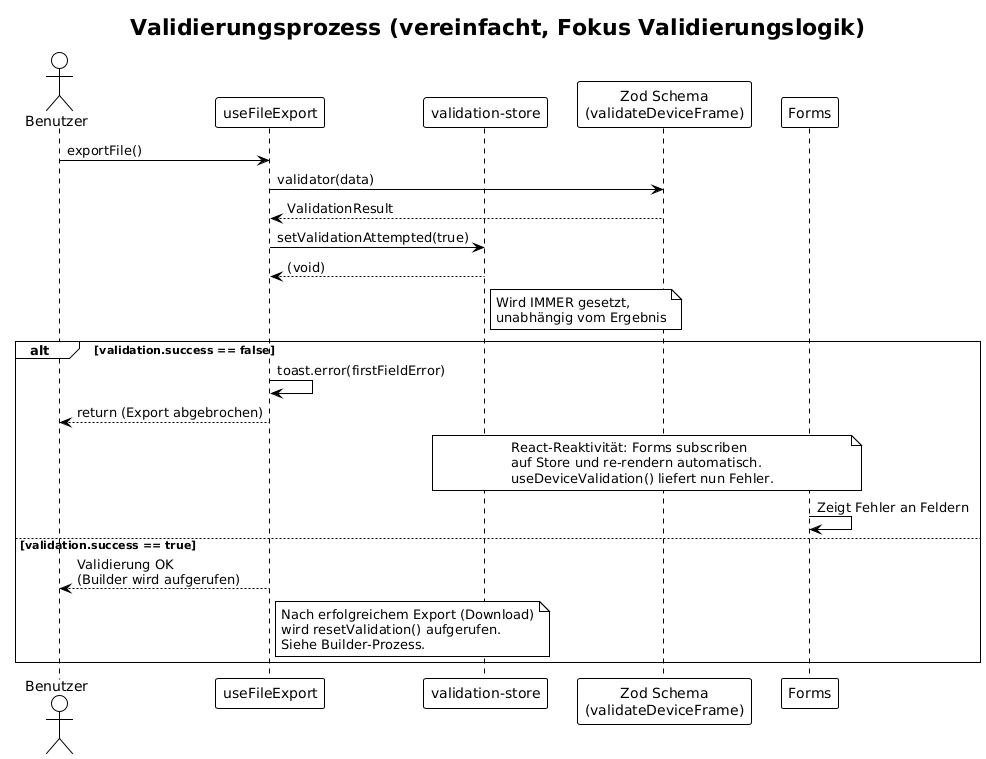
\includegraphics[width=1\textwidth]{ressources/sequenz-diagramm-validation.png}
    \caption{Sequenzdiagramm: Validierungs-Prozess (vereinfacht)}
    \label{fig:validation-flow}
\end{figure}

\newpage

\subsubsection{Zod-Schemas}

Analog zur sektionsbasierten Architektur existiert für jede Sektion eine \code{*-schema.ts} Datei mit dem 
entsprechenden Zod-Schema. Die Übersetzung vom XML-Schema erfolgt systematisch: 
\xmlattr{maxLength="4000"} wird zu \code{z.string().max(4000)}, \xmlattr{maxOccurs="4"} zu \newline
\code{z.array(...).max(4)}, Enumerationen zu \code{z.enum([...])}. \newline

\noindent Abbildung~\ref{fig:xsd-legible-description} und \ref{fig:zod-legible-description} zeigen diese Übersetzung 
am Beispiel \code{LegibleDescription} -- einem Element für mehrsprachige Beschreibungstexte mit begrenzter 
Zeichenzahl.

\begin{figure}[H]
    \centering
    \begin{lstlisting}[language=xsdselective,frame=single,backgroundcolor=\color{gray!10},basicstyle=\ttfamily\scriptsize,breaklines=true]
  <complexType name="LegibleDescription">
    <sequence>
      <element name="textElement">
        <simpleType>
          <restriction base="string">
            <minLength value="0" />
            <maxLength value="4000" />
          </restriction>
        </simpleType>
      </element>
      <element name="language" type="sgr:Language">
      </element>
      <element name="uri" type="anyURI" minOccurs="0">
      </element>
    </sequence>
  </complexType>
  <simpleType name="Language">
    <restriction base="string">
      <enumeration value="de" />
      <enumeration value="en" />
      <enumeration value="fr" />
      <enumeration value="it" />
    </restriction>
  </simpleType>
    \end{lstlisting}
    \caption{XML-Schema: LegibleDescription und Language}
    \label{fig:xsd-legible-description}
\end{figure}

\begin{figure}[H]
    \centering
    \begin{lstlisting}[language=typescriptselective,frame=single,backgroundcolor=\color{gray!10},basicstyle=\ttfamily\scriptsize,breaklines=true]
const LANGUAGE_VALUES_ARRAY = LANGUAGE_VALUES as unknown as [string, ...string[]];

export const legibleDescriptionSchema = z.object({
  textElement: z
    .string({message: "Text element is required"})
    .min(0)
    .max(4000, "Text element cannot exceed 4000 characters"),
  language: z.enum(LANGUAGE_VALUES_ARRAY, {
    message: "Language is required"
  }),
  uri: z.string().optional()
});

// Legible Descriptions Schema (array, maxOccurs="4")
export const legibleDescriptionsSchema = z
  .array(legibleDescriptionSchema)
  .max(4, "Cannot have more than 4 legible descriptions");
    \end{lstlisting}
    \caption{Zod-Schema: legibleDescriptionSchema und legibleDescriptionsSchema}
    \label{fig:zod-legible-description}
\end{figure}

\newpage

% ---------- Builder ----------
\subsection{Builder}
\label{sec:xml-building}

Der Builder ist das Gegenstück zum Mapper: Er transformiert das typisierte Model-Objekt zurück in einen 
XML-String, der dem SGr-Schema entspricht. 

\subsubsection{Prozess}
Nach erfolgreicher Validierung wird der Builder vom Export-Hook 
aufgerufen (Abbildung~\ref{fig:builder-prozessablauf}).

\begin{figure}[H]
    \centering
    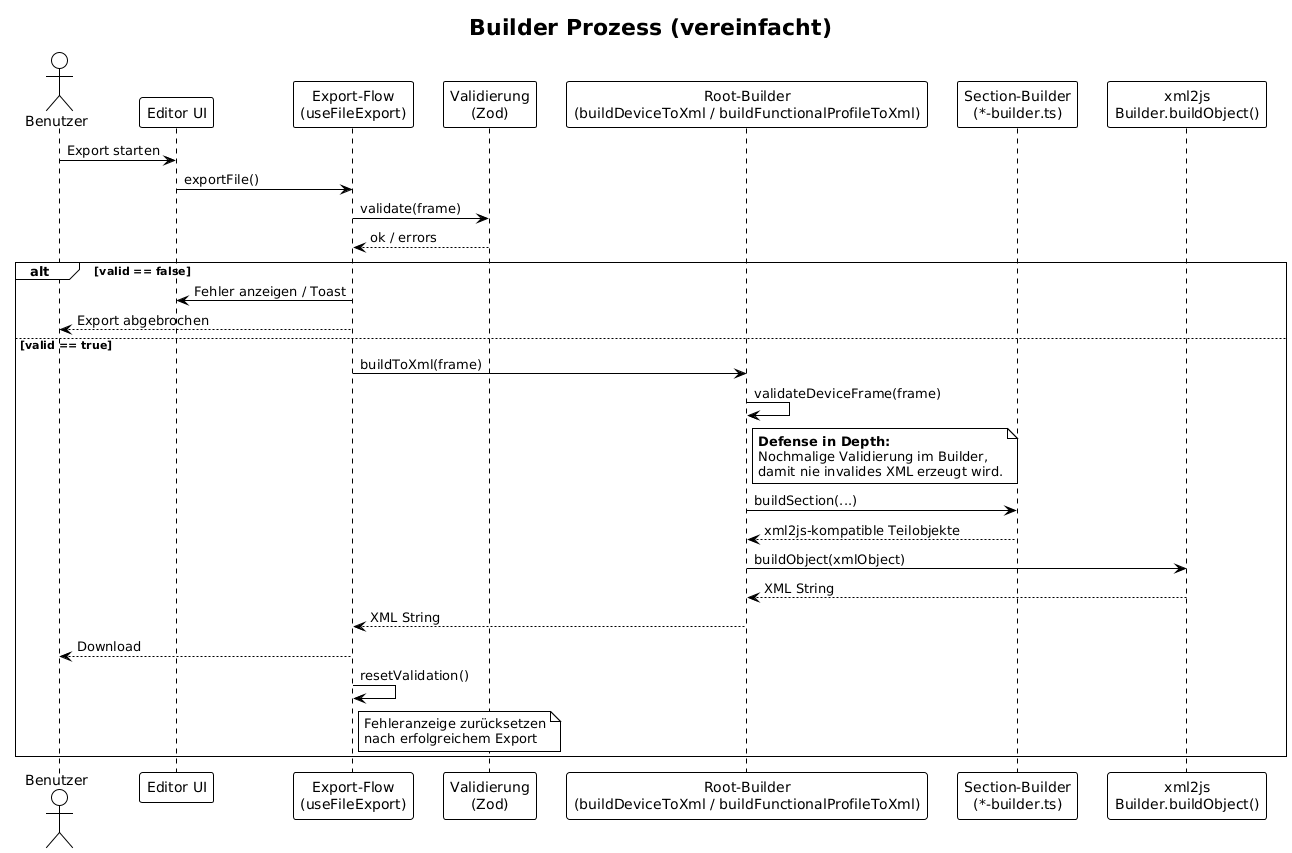
\includegraphics[width=1\textwidth]{ressources/sequenz-diagramm-builder.png}
    \caption{Sequenzdiagramm: Builder-Prozess (vereinfacht)}
    \label{fig:builder-prozessablauf}
\end{figure}

\subsubsection{Builder-Hierarchie}

Die Architektur spiegelt die des Mappers: Ein Root-Builder orchestriert die Transformation und delegiert 
an Section-Builder. Der Root-Builder \code{buildDevice} (Abbildung~\ref{fig:builder-hierarchy}) ruft 
die Section-Builder für die jeweiligen Model-Bereiche auf. Jeder Section-Builder liest die Properties 
aus dem TypeScript-Interface und erzeugt daraus ein xml2js-kompatibles JavaScript-Objekt.

\begin{figure}[H]
    \centering
    \begin{lstlisting}[language=typescriptselective,frame=single,backgroundcolor=\color{gray!10},basicstyle=\ttfamily\scriptsize,breaklines=true]
function buildDevice(device: DeviceFrame): Record<string, unknown> {
  const deviceFrame: Record<string, unknown> = {
    $: { xmlns: "http://www.smartgridready.com/ns/V0/", /* ... */ },
  };

  const identification = buildDeviceIdentification(device);
  deviceFrame.deviceName = identification.deviceName;
  deviceFrame.specificationOwnerIdentification = identification.specificationOwnerIdentification;
  
  deviceFrame.releaseNotes = wrapInArray(buildReleaseNotes(device.releaseNotes));
  deviceFrame.deviceInformation = wrapInArray(buildDeviceInformation(device.deviceInformation));
  deviceFrame.interfaceList = wrapInArray(buildInterfaceList(device.interfaceList));

  return { DeviceFrame: deviceFrame };
}
    \end{lstlisting}
    \caption{Root-Builder: Delegation an Section-Builder}
    \label{fig:builder-hierarchy}
\end{figure}

\noindent Die Section-Builder lesen die Werte aus dem TypeScript-Interface und erzeugen daraus 
xml2js-kompatible Objekte (Abbildung~\ref{fig:section-builder}). \code{wrapInArray} verpackt Werte 
in Arrays, da xml2js diese Struktur für die Serialisierung erwartet.

\begin{figure}[H]
    \centering
    \begin{lstlisting}[language=typescriptselective,frame=single,backgroundcolor=\color{gray!10},basicstyle=\ttfamily\scriptsize,breaklines=true]
// device-information-builder.ts - Section-Builder
export function buildDeviceInformation(info: DeviceInformation): Record<string, unknown> {
  const xml: Record<string, unknown> = {};

  // Pflichtfelder immer setzen
  xml.deviceCategory = wrapInArray(info.deviceCategory);
  xml.isLocalControl = wrapInArray(String(info.isLocalControl));

  // Optionale Felder nur setzen wenn vorhanden
  setOptionalXmlField(xml, "brandName", info.brandName);
  setOptionalXmlField(xml, "softwareRevision", info.softwareRevision);
  // ... weitere optionale Felder

  return xml;
}
    \end{lstlisting}
    \caption{Section-Builder: Interface-Properties zu XML-Objekt}
    \label{fig:section-builder}
\end{figure}

\subsubsection{xml2js-Konfiguration}

Nachdem das JavaScript-Objekt zusammengebaut wurde, serialisiert die xml2js-\code{Builder}-Klasse 
es zu einem XML-String (Abbildung~\ref{fig:xml2js-builder}). Die Optionen steuern das Ausgabeformat:
\begin{itemize}[noitemsep,topsep=0pt]
    \item \code{pretty: true} -- XML wird mit Einrückungen formatiert für bessere Lesbarkeit.
    \item \code{cdata: true} -- Textfelder mit Sonderzeichen (\code{<}, \code{>}, \code{\&}) werden 
          in CDATA-Blöcke eingepackt, um die Zeichen zu schützen.
    \item \code{xmldec} -- Generiert die XML-Deklaration (\code{<?xml version="1.0"?>}).
\end{itemize}

\begin{figure}[H]
    \centering
    \begin{lstlisting}[language=typescriptselective,frame=single,backgroundcolor=\color{gray!10},basicstyle=\ttfamily\scriptsize,breaklines=true]
const xmlObject = buildDevice(device);

const builder = new Builder({
  xmldec: { version: "1.0", encoding: "UTF-8" },
  renderOpts: { pretty: true, indent: "  " },
  headless: false,
  cdata: true,
});

const xmlString = builder.buildObject(xmlObject);
    \end{lstlisting}
    \caption{Builder-Konfiguration für xml2js}
    \label{fig:xml2js-builder}
\end{figure}

\noindent Der resultierende XML-String wird dem Benutzer als Download angeboten.

\newpage

% ---------- Future Work ----------
\subsection{Future Work}
\label{sec:future-work}

Während der Entwicklung wurden Bereiche identifiziert, die in zukünftigen Iterationen 
verbessert werden könnten. Nachfolgend werden diese Bereiche beschrieben.

\subsubsection{Store-Optimierung}

Die aktuelle Store-Architektur verwendet zwei monolithische Zustand-Stores (\code{useDeviceStore} und 
\code{useProfileStore}), die jeweils zahlreiche hierarchisch verschachtelte Slices kombinieren. 
Obwohl diese Architektur funktional ist und durch Debouncing sowie selektive Subscriptions bereits 
optimiert wurde, ergeben sich bei wachsender Komplexität potenzielle Verbesserungsmöglichkeiten. \newline

\noindent\textbf{Identifizierte Probleme:} Alle Daten in einem Store können zu unnötigen Re-Renders 
führen und erschweren Wartbarkeit sowie Debugging. Die tiefe Verschachtelung (>80 Slices für Device) 
fragmentiert zudem den Code und erschwert die Navigation. \newline

\noindent\textbf{Empfohlene Massnahmen:} Statt eines grossen Stores könnten separate, fokussierte 
Stores für logische Bereiche erstellt werden (\textit{Store-Splitting}). Für verschachtelte Listen 
wie FunctionalProfiles und DataPoints könnte ein Provider-Pattern mit React Context verwendet werden 
(\textit{Context-basierte Stores}). Zusätzlich könnten kritische Sektionen separat mit 
unterschiedlichen Debounce-Zeiten gespeichert werden (\textit{Selektive Persistenz}). \newline

\noindent Für zukünftige Erweiterungen oder bei Performance-Problemen mit grösseren Datenmengen sollte 
das Store-Splitting priorisiert werden.

\newpage

% ---------- Fazit ----------
\section{Fazit}

% ---------- Einsatz von KI-Unterstützung ----------
\subsection{Einsatz von KI-Unterstützung}

Durch die sektionsbasierte Architektur entstanden viele strukturell ähnliche Dateien: 
Jede Sektion braucht ein eigenes Formular, einen Mapper, einen Builder, ein Schema und einen Store-Slice. 
Diese repetitive Arbeit manuell zu erledigen, wäre ineffizient gewesen – weshalb wir früh auf KI-gestützte Werkzeuge gesetzt haben.
Wir nutzten die KI vor allem als Schreib- und Strukturhilfe: Anforderungen und Patterns wurden beschrieben,
das Resultat anschliessend geprüft und an die bestehende Codebasis angepasst. Als Entwicklungsumgebung nutzten wir den Editor
\code{Cursor}; als KI-Modell kam \code{Claude Opus 4.5} zum Einsatz.
\newline
Um die Zusammenarbeit mit der KI nachvollziehbar und wiederholbar zu machen, haben wir zwei Prompt-Guides erstellt:
\textbf{„Shared Sektionen“} und \textbf{„Single Sektionen“}
(siehe Anhang~\ref{app:prompts-single}). Die Guides unterscheiden
zwischen Shared-Sektionen (mehrmals in einem Kontext und/oder in beiden Kontexten) und Single-Sektionen (genau einmal in genau einem Kontext)
und liefern dafür jeweils strukturierte Prompt-Vorlagen
für Factory, Schema, Store-Slice, Form, Mapper und Builder.


% ---------- Schlussfolgerung ----------
\subsection{Schlussfolgerung}

Im Rahmen dieses Projekts ist ein funktionaler Prototyp eines web-basierten Deklarations-Tools für SmartGridready 
entstanden. Damit können Produktbeschreibungen und Funktionsprofile erstellt, importiert, bearbeitet und wieder 
exportiert werden. Unser Ziel, die Gesamtheit des XML-Schemas in einer geführten Oberfläche abbilden zu können, 
wurde damit erreicht.

Aus unserer Sicht ist besonders die Benutzeroberfläche gelungen: Statt mit XML im Texteditor zu arbeiten, werden 
die Inhalte hinter einer klar strukturierten Eingabemaske versteckt. Dadurch wird die Hürde beim Erstellen und Pflegen 
von Deklarationen reduziert. Diese Einschätzung basiert jedoch auf unserer Entwicklungserfahrung; als 
nächster Schritt sollten User-Tests mit Personen durchgeführt werden, die in der Praxis Deklarationen erstellen 
und bearbeiten. So kann überprüft werden, ob das Tool im Alltag tatsächlich verständlich ist und den Workflow 
spürbar verbessert.

% ---------- Projektreflexion ----------
\subsection{Projektreflexion}

Das Projekt war für uns sehr spannend, aber auch sehr herausfordernd. Der Einstieg war nicht einfach, weil die 
SmartGridready-Thematik neu für uns war und wir uns zuerst in die Spezifikation sowie in die bestehenden 
Deklarationen einarbeiten mussten. Gerade zu Beginn wirkte die Menge an Regeln und Varianten im Schema 
überwältigend.

Rückblickend haben wir die Komplexität unterschätzt. Sobald ein Schema-Element eingepflegt war, musste es 
konsequent in der Eingabemaske sowie in Import/Export, Store und Validierung mitgezogen werden. Die Sektionsbasierte 
Strukturierung war hilfreich, erforderte aber einen ständigen Abgleich mit anderen Sektionen um Patterns konsistent zu halten.

% ---------- Dank ----------
\subsection{Dank}

Ein grosser Dank geht an unsere Coaches Jürg Luthiger und Matthias Krebs für den Support und das konstante 
Feedback. Ihre Tipps und Rückmeldungen haben uns in der Ausrichtung des Projekts und in der Umsetzung immer 
wieder weitergeholfen.

\newpage

% ---------- Literaturverzeichnis ----------
\section{Literaturverzeichnis}

\begin{enumerate}[label={[\arabic*]}]
    \item SmartGridready, ``SGrSpecifications''. GitHub Repository. [Online]. Verfügbar unter: 
          \href{https://github.com/SmartGridready/SGrSpecifications}{Link}
    
    \item SmartGridready, ``SmartGridready -- Offene Kommunikation für das intelligente Stromnetz''. 
          [Online]. Verfügbar unter: \href{https://smartgridready.ch/}{Link}
    
    \item Wikipedia, ``XML Schema''. [Online]. Verfügbar unter: 
          \href{https://de.wikipedia.org/wiki/XML_Schema}{Link}
    
    \item Vercel, ``Next.js -- The React Framework for the Web''. [Online]. Verfügbar unter: 
          \href{https://nextjs.org/}{Link}
    
    \item pmndrs, ``Zustand -- A small, fast and scalable bearbones state-management solution''. 
          [Online]. Verfügbar unter: \href{https://github.com/pmndrs/zustand}{Link}
    
    \item Microsoft, ``TypeScript -- JavaScript With Syntax For Types''. [Online]. Verfügbar unter: 
          \href{https://www.typescriptlang.org/}{Link}
    
    \item L. Moesinger, ``xml2js -- Simple XML to JavaScript object converter''. npm. [Online]. 
          Verfügbar unter: \href{https://www.npmjs.com/package/xml2js}{Link}
    
    \item C. Hofer, ``Zod -- TypeScript-first schema validation with static type inference''. 
          [Online]. Verfügbar unter: \href{https://zod.dev/}{Link}
    
    \item shadcn, ``shadcn/ui -- Beautifully designed components built with Radix UI and Tailwind CSS''. 
          [Online]. Verfügbar unter: \href{https://ui.shadcn.com/}{Link}
\end{enumerate}

% ---------- Abbildungsverzeichnis ----------
\newpage
\appendix

% Appendix: A Anhang, A1 Prompt Guides, B Abbildungsverzeichnis
\renewcommand{\thesubsection}{\thesection\arabic{subsection}}

\section{Anhang}

\subsection{Prompt Guides}
\label{sec:ai-prompts}

\begin{itemize}
    \item \label{app:prompts-shared}\textbf{\href{https://gitlab.fhnw.ch/ip5-smartgridready/docs/-/blob/main/Report/attachments/prompts-shared.md}{KI-Prompts: Shared-Sektionen}}\\
    Prompts und Patterns für Sektionen, die mehrmals in einem Kontext und/oder in beiden Kontexten vorkommen
    (Device \textbf{und}/oder Functional Profile).

    \item \label{app:prompts-single}\textbf{\href{https://gitlab.fhnw.ch/ip5-smartgridready/docs/-/blob/main/Report/attachments/prompts-single.md}{KI-Prompts: Single Sektionen}}\\
    Prompts und Patterns für Sektionen, die genau einmal in genau einem Kontext vorkommen (Device \textbf{oder} Functional Profile)
    und nicht als Shared-Komponente abstrahiert werden müssen.
\end{itemize}

% ---------- Abbildungsverzeichnis ----------
\newpage
\section{Abbildungsverzeichnis}
\renewcommand{\listfigurename}{}
\listoffigures

\end{document}
 